\documentclass[11pt,a4paper,twoside]{scrreprt}
\KOMAoptions{open=right, cleardoublepage=empty}

% ---------- Base encoding & fonts ----------
\usepackage[T1]{fontenc}
\usepackage[utf8]{inputenc}
\usepackage{lmodern}
\usepackage{microtype}
\usepackage{accsupp}  % lets us control ActualText for copy/paste

\DeclareRobustCommand{\copyspace}{%
  \BeginAccSupp{ActualText= }%  % what the clipboard receives (a real U+0020)
  \kern0pt\ %                    % what is drawn (a normal space)
  \EndAccSupp
}
% ---------- Graphics & links ----------
\usepackage{graphicx}
\usepackage[dvipsnames]{xcolor}
\usepackage{hyperref}
\hypersetup{
  colorlinks=true,
  linkcolor=blue!60!black,
  urlcolor=blue!60!black,
  citecolor=blue!60!black
}

% ---------- Lists, tables, floats ----------
\usepackage{enumitem}                % for [nosep]
\usepackage{booktabs}                % \toprule etc.
\usepackage{float}                   % [H] placement
\usepackage{tabularx,array}
\renewcommand{\arraystretch}{1.15}

% ---------- KOMA (safe if class is scrreprt/scrartcl) ----------
\makeatletter
\@ifundefined{KOMAClassName}{}{%
  \KOMAoptions{
    DIV=14,
    BCOR=0mm,
    headinclude=true,
    footinclude=false
  }%
}
\makeatother

% ---------- Numbering & ToC ----------
\setcounter{secnumdepth}{3}
\setcounter{tocdepth}{3}             % show down to subsubsection in ToC
\renewcommand\thesection{\arabic{section}}
\renewcommand\thesubsection{\thesection.\arabic{subsection}}
\renewcommand\thesubsubsection{\thesubsection.\arabic{subsubsection}}

% ---------- Small helpers ----------
\newcommand{\keil}{\textbf{Keil uVision5}}
\providecommand{\tightlist}{\setlength{\itemsep}{0pt}\setlength{\parskip}{0pt}}

% ---------- Listings: ARM assembly (colors + top/bottom rules only) ----------
\usepackage{listings}
\usepackage{listingsutf8}

% Palette
\definecolor{AsmMnemonic}{HTML}{005CC5}   % blue
\definecolor{AsmDirective}{HTML}{6F42C1}  % purple
\definecolor{AsmCond}{HTML}{D73A49}       % red
\definecolor{AsmRegister}{HTML}{22863A}   % green
\definecolor{AsmComment}{HTML}{6A737D}    % gray
\definecolor{AsmLineNo}{HTML}{9AA0A6}     % light gray
\definecolor{AsmRule}{HTML}{C0C4C8}       % rule color

% Language
\lstdefinelanguage{Assembler}{
  % Mnemonics (include S-suffixed forms and conditional branch forms)
  morekeywords={
    ADC,ADCS,ADD,ADDS,ADR,AND,ANDS,ASR,ASRS,
    B,BEQ,BNE,BCS,BHS,BCC,BLO,BMI,BPL,BVS,BVC,BHI,BLS,BGE,BLT,BGT,BLE,BAL,
    BL,BLX,BX,
    CBNZ,CBZ,CLZ,CMP,CMN,
    EOR,EORS,
    ISB,
    LDM,LDR,LDRB,LDRH,
    LSL,LSLS,LSR,LSRS,
    MOV,MOVS,MOVT,MOVW,MSR,MRS,
    MUL,MULS,
    NOP,
    ORR,ORRS,
    POP,PUSH,
    REV,REV16,REVSH,
    ROR,RORS,
    SBC,SBCS,
    SEV,
    STM,STR,STRB,STRH,
    SUB,SUBS,
    TBB,TBH,TST,
    UXTB,UXTH,UXTB16,
    WFE,WFI,
    YIELD,
    BKPT
  },
  % Directives
  morekeywords=[2]{AREA,ALIGN,DCD,DCB,DCW,EXPORT,IMPORT,ENTRY,END,SPACE,KEEP,WEAK,LTORG,PROC,ENDP},
  % Condition-code tokens (when written separately; kept for completeness)
  morekeywords=[3]{EQ,NE,CS,HS,CC,LO,MI,PL,VS,VC,HI,LS,GE,LT,GT,LE,AL},
  morecomment=[l]{;},
  sensitive=true
}
\lstdefinelanguage[ARM]{Assembler}[]{Assembler}{}


\lstdefinestyle{labcode}{
  language={[ARM]Assembler},
  inputencoding=utf8,
  basicstyle=\ttfamily\small,  % inconsolata will be used
  columns=fixed,               % fixed-width columns -> real spaces in PDF
  keepspaces=true,             % preserve all spaces (incl. leading)
  tabsize=4,                   % set to the width you expect; or convert tabs to spaces
  showstringspaces=false,
  upquote=true,
  keywordstyle={\color{AsmMnemonic}\bfseries},
  keywordstyle=[2]{\color{AsmDirective}\bfseries},
  keywordstyle=[3]{\color{AsmCond}\bfseries},
  commentstyle={\itshape\color{AsmComment}},
  emph={R0,R1,R2,R3,R4,R5,R6,R7,R8,R9,R10,R11,R12,SP,LR,PC,
        APSR,IP,PSP,MSP,xPSR},
  emphstyle={\color{AsmRegister}\bfseries},
  showstringspaces=false,
  tabsize=2,
  keepspaces=true,
  columns=fullflexible,
  % line breaking
  breaklines=true,
  breakatwhitespace=true,
  % frame: top & bottom only
  frame=lines,
  rulecolor={\color{AsmRule}},
  xleftmargin=2em,
  framexleftmargin=2em,
  % line numbers
  % line numbers disabled
  % float control
  float,
  floatplacement=H,
  captionpos=b,
}
\lstset{style=labcode}
\usepackage{amsmath}
\usepackage{tcolorbox}
\usepackage{tikz}
\usetikzlibrary{positioning,arrows.meta,decorations.pathreplacing}
\usepackage{subcaption} % or subfig if you prefer
% ---------- Chapter-level ToCs ----------

% ---------- Tables of contents ----------
\usepackage{etoc}  % local ToCs that inherit the same style as \tableofcontents
\usepackage{titletoc}  % for \titlecontents command
% ---------- Cover page config ----------
% If you use an SVG logo, keep this. If you prefer PNG/PDF, you may omit.
\usepackage{svg} % requires --shell-escape or inkscape; else convert logo to PDF/PNG

% Editable cover fields

% ---- Technical manual title page helpers ----
% Logo is expected at assets/<name>.svg; adjust if needed.
\svgpath{{resources/}} % where the logo lives

\providecommand{\LOGONAME}{birzeit-logo} % base name, no extension
\providecommand{\DEPARTMENT}{Department of Electrical \& Computer Engineering}
\providecommand{\COURSENUM}{ENCS4110}
\providecommand{\COURSENAME}{Computer Design Laboratory}
% ---- Cover defaults (override as needed) ----
\providecommand{\ManualSubtitle}{Laboratory Manual}

% Semantic version pieces (or set \ManualVersion directly)
\providecommand{\ManualVersionMajor}{1}
\providecommand{\ManualVersionMinor}{0}
\providecommand{\ManualVersionPatch}{0}
\providecommand{\ManualVersion}{v\ManualVersionMajor.\ManualVersionMinor.\ManualVersionPatch}
\newcommand{\MonthYear}{%
  \ifcase\month
  \or January\or February\or March\or April\or May\or June%
  \or July\or August\or September\or October\or November\or December
  \fi~\the\year
}
% Local ToC etc. can stay as-is. Ensure svg path is set:
\makeatletter
\newcommand{\maketechnicaltitlepage}{%
  \begin{titlepage}
    \thispagestyle{empty}

    % --- Top: logo + department + course ---
    \vspace*{1.2cm}
    \begin{center}
      \IfFileExists{assets/\LOGONAME.pdf}
        {\includegraphics[width=.80\textwidth]{assets/\LOGONAME.pdf}}
        {\includesvg[width=.80\textwidth,inkscapelatex=false]{\LOGONAME}}

      \vspace{0.3cm}
      {\large \DEPARTMENT\par}
      {\large \COURSENUM\;--\;\COURSENAME\par}
    \end{center}

    % --- Middle: centered Title + Subtitle ONLY ---
    \vspace{1.5cm}
    \begin{center}
      {\Huge\bfseries \@title\par}
      \vspace{0.35cm}
      {\Large \ManualSubtitle\par}
    \end{center}
    \vfill

    % --- Bottom-left: Version + Date ---
    \begin{flushleft}
      {\large \textbf{Version:} \ManualVersion}\\[0.2cm]
        {\large \textbf{Date:} \MonthYear}
    \end{flushleft}
  \end{titlepage}%
}
\makeatother

% ---- titletoc formatting: Tufte-ish, robust ----
\usepackage{titletoc}

\titlecontents{part}%
  [0pt]% distance from left margin
  {\addvspace{0.25\baselineskip}}% above (global formatting of entry)
  {\allcaps{Part~\thecontentslabel}\quad}% before w/ label (label = ``Part I'')
  {\allcaps{Part~\thecontentslabel}\allcaps}% before w/o label
  {}% filler and page (leaders and page num)
  [\vspace*{0.5\baselineskip}]% after

\titlecontents{chapter}%
    [4em]% distance from left margin
    {}% above (global formatting of entry)
    {\contentslabel{2em}\textit}% before w/ label (label = ``Chapter 1'')
    {\hspace{0em}\textit}% before w/o label
    {\qquad\thecontentspage}% filler and page (leaders and page num)
    [\vspace*{0.5\baselineskip}]% after
%%%% End additional code by Kevin Godby


% Silent part: adds a numbered Part entry to the ToC, prints nothing
% --- ToC-only “Part” entry (no heading printed, no hyperlink in ToC) ---
\makeatletter
\newcommand{\toconlypart}[1]{%
  \clearpage                 % keep if you want a clean break; remove if not
  \refstepcounter{part}%     % step the Part counter (I, II, …)
  % Write a plain (non-hyperlinked) contents line: 4th arg = link target -> empty
  \addtocontents{toc}{%
    \protect\contentsline{part}{\protect\numberline{\thepart}#1}{\thepage}{}%
  }%
  % Optional: set header marks if you use \leftmark/\rightmark
  \markboth{Part \thepart\quad #1}{}%
}
\makeatother


\usepackage{bytefield}
\usepackage[table]{xcolor} % for light gray shading
\usepackage{needspace}


\usepackage{graphicx} % for \resizebox
\usepackage{calc}     % for \widthof
\usepackage{bytefield}

% measure once
\newlength{\pfbit}
\settowidth{\pfbit}{\tiny PF0} % or {\scriptsize PF0} if you prefer

\providecommand{\allcaps}[1]{\MakeUppercase{#1}}




\providecommand{\LOGONAME}{birzeit-logo} % base name, no extension
\providecommand{\DEPARTMENT}{Department of Electrical \& Computer Engineering}
\providecommand{\COURSENUM}{ENCS4110}
\providecommand{\COURSENAME}{Computer Design Laboratory}
\title{Laboratory Manual}
\renewcommand{\ManualSubtitle}{ARM Cortex-M4 (TM4C123) — Assembly}
\renewcommand{\ManualVersionMajor}{1}
\renewcommand{\ManualVersionMinor}{0}
\renewcommand{\ManualVersionPatch}{0}

\date{\today}

\begin{document}

\KOMAoptions{twoside=false}\recalctypearea
\maketechnicaltitlepage
\KOMAoptions{twoside=true}\recalctypearea
% Global ToC: chapters only
\cleardoublepage
\begingroup
\setcounter{tocdepth}{0} % parts and chapters only
\tableofcontents
\endgroup
\cleardoublepage

\toconlypart{ARM Cortex-M4 Assembly Programming}
\chapter{ARM Cortex-M4 Assembly Fundamentals}

\section*{Learning Objectives}
\begin{itemize}[nosep]
  \item Describe the Cortex-M4 register set, xPSR flags, and ARMv7-M memory map.
  \item Write and assemble a minimal ARM program with a vector table and \texttt{Reset\_Handler}.
  \item Use core data-processing, shift/rotate, and compare/test instructions.
  \item Apply conditional execution with condition codes (e.g., \texttt{ADDEQ}, \texttt{BNE}).
  \item Debug in \keil: set breakpoints, single-step, inspect registers/memory, and interpret flags.
\end{itemize}

\section*{Experiment Overview}
This experiment introduces low-level programming on the Cortex-M4. You will build a minimal startup image, practice common data-processing and control-flow instructions, and use the \keil\ debugger to observe register and memory effects while stepping through code. By the end, you will be able to implement and test short assembly routines that manipulate data and make decisions based on condition flags.

\newpage
\tableofcontents
\newpage
\section{Theoretical Background}
\subsection{Cortex-M4 Architecture}
\subsubsection{Registers Overview}
The Cortex-M4 architecture includes a set of general-purpose registers (R0-R12), a stack pointer (SP), a link register (LR), a program counter (PC), and a program status register (xPSR), all of which are 32-bit registers. The general-purpose registers are used for data manipulation and temporary storage during program execution. The SP is used to manage the call stack, while the LR holds the return address for function calls. The PC points to the next instruction to be executed, and the xPSR contains flags and status information about the processor state.
\paragraph{Program Status Register (xPSR)}
holds the current state of the processor, including condition flags (Negative, Zero, Carry, Overflow), interrupt status, and execution state. These flags are updated based on the results of arithmetic and logical operations, allowing for conditional branching and decision-making in programs.

\subsubsection{Memory Mapping}
The Cortex-M4 uses a flat memory model, where all memory locations are accessible through a single address space. This model simplifies programming and allows for efficient access to data and instructions. The memory is divided into several regions, including code memory (for storing instructions), data memory (for storing variables), and peripheral memory (for interfacing with hardware components). The architecture supports both little-endian and big-endian data formats, with little-endian being the default.
\begin{table}[H]
\centering
\caption{Cortex-M4 Memory Regions (ARMv7-M)}
\begin{tabularx}{\linewidth}{@{}p{0.20\linewidth}p{0.30\linewidth}X@{}}
\toprule
\textbf{Region} & \textbf{Address Range} & \textbf{Description} \\
\midrule
Code            & \texttt{0x00000000}--\texttt{0x1FFFFFFF} & Flash memory for program code \\[0.5ex]
SRAM            & \texttt{0x20000000}--\texttt{0x3FFFFFFF} & On-chip static RAM for data \\[0.5ex]
Peripheral      & \texttt{0x40000000}--\texttt{0x5FFFFFFF} & Memory-mapped peripheral registers \\[0.5ex]
External RAM    & \texttt{0x60000000}--\texttt{0x9FFFFFFF} & External RAM (if implemented) \\[0.5ex]
External Device & \texttt{0xA0000000}--\texttt{0xDFFFFFFF} & External devices/memory (if implemented) \\[0.5ex]
Private Peripheral Bus & \texttt{0xE0000000}--\texttt{0xE00FFFFF} & Cortex-M4 internal peripherals  (NVIC, SysTick, MPU, SCB)\\
System          & \texttt{0xE0100000}--\texttt{0xFFFFFFFF} & System region (reserved/system-level) \\
\bottomrule
\end{tabularx}
\end{table}


\subsection{Assembly Language Basics}

Assembly language is a low-level programming language that provides a direct correspondence between human-readable instructions and the machine code executed by the processor. Each instruction encodes a specific operation, such as moving data, performing arithmetic or logic, or altering control flow. Because it maps so closely to hardware, assembly allows precise control of system resources and is commonly used in performance-critical routines or when direct access to hardware is required.

Assembly programs are typically composed of three main elements: \emph{instructions}, \emph{directives}, and \emph{labels}.

\paragraph{Instructions}  
Instructions are the executable commands that the CPU carries out. Examples include data movement (\texttt{MOV}), arithmetic (\texttt{ADD}, \texttt{SUB}), logical operations (\texttt{AND}, \texttt{ORR}), and control flow (\texttt{B}, \texttt{BL}). Each instruction directly translates to one or more machine code opcodes and determines the actual behavior of the program.

\paragraph{Directives}  
Directives are commands to the assembler that guide how source code is translated into machine code but do not generate instructions themselves. Common examples include \texttt{AREA} (define a code or data section), \texttt{ALIGN} (align data to memory boundaries), \texttt{DCD} (allocate and initialize a word of storage), and \texttt{EXPORT} (export a symbol for linking). Directives organize program layout, control memory allocation, and manage symbol visibility.

\paragraph{Labels}  
Labels are symbolic names that mark specific locations in code or data. They act as targets for jumps and branches or as references for data access. Labels improve program readability and maintainability by avoiding hard-coded addresses. For instance, a label like \texttt{loop\_start} can be used as the destination of a branch instruction, and the assembler automatically computes the correct relative address.
\subsubsection{Instruction Set Overview}
The ARM Cortex-M4 instruction set is a subset of the ARMv7-M architecture, designed for efficient execution in embedded systems. It includes a variety of instructions for data processing, memory access, and control flow. Key categories of instructions include:
\hfill
\begin{itemize}[nosep]
    \item \textbf{Data Processing Instructions}: These include arithmetic operations (e.g., \texttt{ADD}, \texttt{SUB}), logical operations (e.g., \texttt{AND}, \texttt{ORR}), and data movement instructions (e.g., \texttt{MOV}, \texttt{MVN}).
    \item \textbf{Load and Store Instructions}: Instructions like \texttt{LDR} (load register) and \texttt{STR} (store register) are used to transfer data between registers and memory.
    \item \textbf{Branch Instructions}: Control flow is managed using branch instructions such as \texttt{B} (branch), \texttt{BL} (branch with link), and conditional branches like \texttt{BEQ} (branch if equal).
    \item \textbf{Special Instructions}: These include instructions for system control, such as \texttt{NOP} (no operation), \texttt{WFI} (wait for interrupt), and instructions for manipulating the stack and handling exceptions.
\end{itemize}
\subsubsection{General Instruction Format}

Assembly source lines generally follow this shape:

\[
\texttt{[label]} \quad \texttt{OPCODE\{<cond>\}\{S\}} \quad \texttt{operands} \quad \texttt{\color{lightgray}; comment}
\]

where curly braces \texttt{\{\}} denote optional components, and:
\begin{itemize}[nosep]
  \item \texttt{label}: optional symbolic name marking the current address.
  \item \texttt{OPCODE}: instruction mnemonic (e.g., \texttt{ADD}, \texttt{MOV}, \texttt{B}).
  \item \texttt{<cond>}: optional condition code (e.g., \texttt{EQ}, \texttt{NE}, \texttt{LT}, \texttt{GE}) that predicates execution.
  \item \texttt{S}: optional suffix indicating whether to update the condition flags (e.g., \texttt{ADDS}).
  \item \texttt{operands}: registers, immediates, or memory operands (e.g., \texttt{R0, R1, \#1} or \texttt{[R2]}).
  \item Anything after a semicolon (\texttt{;}) is a comment ignored by the assembler.
\end{itemize}

\begin{lstlisting}[caption={Instruction format example}]
loop_start   ADDS   R0, R0, #1      ; R0 = R0 + 1, update flags (N,Z,C,V)
             CMP    R0, #10         ; compare R0 with 10 (sets flags)
             BLT    loop_start      ; branch if R0 < 10 (uses flags)
\end{lstlisting}
\subsubsection{Conditional Execution}

Most ARM instructions can be made \emph{conditional} by appending a two-letter
\emph{condition code} to the mnemonic (e.g., \texttt{ADDEQ}, \texttt{ADDNE}).
The instruction is executed only if the condition evaluates true based on the
\texttt{xPSR} flags $N$ (negative), $Z$ (zero), $C$ (carry), and $V$ (overflow).
When no condition is supplied, the default is \texttt{AL} (always).

\begin{table}[H]
\centering
\caption{Common ARM Condition Codes}
\small
\begin{tabularx}{0.72\linewidth}{@{}l l X@{}}
\toprule
\textbf{Cond.} & \textbf{Meaning} & \textbf{Description} \\
\midrule
EQ  & Equal                     & Execute if $Z=1$. \\
NE  & Not equal                 & Execute if $Z=0$. \\
CS/HS & Carry set / Unsigned higher or same & Execute if $C=1$. \\
CC/LO & Carry clear / Unsigned lower        & Execute if $C=0$. \\
MI  & Minus (negative)          & Execute if $N=1$. \\
PL  & Plus (non-negative)       & Execute if $N=0$. \\
VS  & Overflow set              & Execute if $V=1$. \\
VC  & Overflow clear            & Execute if $V=0$. \\
HI  & Unsigned higher           & Execute if $C=1$ \emph{and} $Z=0$. \\
LS  & Unsigned lower or same    & Execute if $C=0$ \emph{or} $Z=1$. \\
GE  & Greater or equal (signed) & Execute if $N=V$. \\
LT  & Less than (signed)        & Execute if $N\neq V$. \\
GT  & Greater than (signed)     & Execute if $Z=0$ \emph{and} $N=V$. \\
LE  & Less or equal (signed)    & Execute if $Z=1$ \emph{or} $N\neq V$. \\
AL  & Always                    & Always execute (default if no condition). \\
NV  & Never                     & Reserved / do not use. \\
\bottomrule
\end{tabularx}
\end{table}

\paragraph{Example:}
\begin{lstlisting}[caption={Using conditional-suffix mnemonics},label={lst:cond-exec}]
        CMP     R0, #0          ; set flags from (R0 - 0)
        ADDEQ   R1, R1, #1      ; if Z==1: R1++
        ADDNE   R2, R2, #1      ; if Z==0: R2++
\end{lstlisting}

\subsubsection{Barrel Shifter}
    
The barrel shifter is a hardware feature that allows …is a hardware feature that allows for efficient shifting and rotating of register values as part of data processing instructions. It can perform operations such as logical shifts (left or right), arithmetic shifts, and rotations on the second operand (\texttt{Operand2}) before it is used in the instruction without wasting extra instructions or cycles.

\noindent Examples of barrel shifter usage:
\begin{lstlisting}[caption={Barrel shifter examples}]
    ADD    R0, R2, R1, LSL #2    ; R0 = R2 + (R1 << 2) using barrel shifter
    SUB    R3, R4, R5, LSR #1    ; R3 = R4 - (R5 >> 1) using barrel shifter
    ORR    R6, R7, R8, ROR #3    ; R6 = R7 | (R8 rotated right by 3)
\end{lstlisting}

\newpage
\subsection{Basic Program Template (Boilerplate)}

The minimal skeleton below shows a valid vector table in a \texttt{READONLY} \texttt{RESET} area, a \texttt{READWRITE} data area for variables, and a code area with the \texttt{Reset\_Handler} entry point.

\begin{lstlisting}[caption={Cortex-M4 boilerplate with READWRITE data}]
        AREA    RESET, CODE, READONLY     ; Vector table lives in read-only code
        EXPORT  __Vectors                 ; Make symbol visible to the linker
__Vectors
        DCD     0x20001000                ; Initial SP value (top of stack in SRAM)
        DCD     Reset_Handler             ; Reset vector: entry address
        ALIGN        
        ; -------------------- Read-Write Data --------------------
        AREA    M_DATA, DATA, READWRITE   ; Variables go here (RAM)
        EXPORT  COUNT                     ; Export if referenced by other modules
COUNT   DCD     0                         ; Initialized RW variable (word)
BUF     SPACE   16                        ; Uninitialized RW buffer (16 bytes)
        ALIGN        
        ; -------------------- Application Code -------------------
        AREA    MYCODE, CODE, READONLY
        ENTRY
        EXPORT  Reset_Handler
Reset_Handler
        ; Example: COUNT++ and store to BUF[0]
        LDR     R0, =COUNT                ; R0 <- &COUNT
        LDR     R1, [R0]                  ; R1 <- COUNT
        ADDS    R1, R1, #1                ; R1 = R1 + 1 (update flags)
        STR     R1, [R0]                  ; COUNT <- R1        
        LDR     R2, =BUF                  ; R2 <- &BUF
        STRB    R1, [R2]                  ; BUF[0] <- (low byte of R1)
STOP    B       STOP                      ; Stay here forever
        END
\end{lstlisting}

\paragraph{What each directive does}
\begin{itemize}[nosep]
  \item \texttt{AREA <name>, CODE|DATA, READONLY|READWRITE}:
        defines a section. Put the vector table and program text in \texttt{CODE, READONLY};
        put variables in \texttt{DATA, READWRITE}.
  \item \texttt{EXPORT <symbol>}: makes a label visible to the linker/other modules.
  \item \texttt{DCD, DCW, DCB <values>}: allocate and initialize words, halfwords, or bytes.
  \item \texttt{SPACE <n>}: reserve \textit{n} bytes of uninitialized storage in RAM.
  \item \texttt{ALIGN}: align to a suitable boundary (commonly 4 bytes for words).
  \item \texttt{ENTRY}: mark the entry point of the image for the toolchain.
  \item \texttt{END}: end of source file.
\end{itemize}

\paragraph{Notes}
\begin{itemize}[nosep]
    \item The first two words in \texttt{\_\_Vectors} must be the initial stack pointer value and the address of \texttt{Reset\_Handler}.
    \item The assembler/linker places sections in appropriate memory regions based on the target device and linker script.
    \item Labels must start at the beginning of the line (no indentation), while instructions and directives should be indented for proper assembly.
    \item Variables in \texttt{READWRITE} areas are initialized to zero by default. While you can specify initial values using directives like \texttt{DCD}, the linker will place these in flash and copy them to RAM during startup, or they may be zeroed out during RAM initialization.
\end{itemize}

\newpage
\section{Procedure}
\subsection{Setting Up the Keil uVision5 Environment}
Make sure you have the \keil\ IDE installed on your computer. If not, download and install it from the official Keil website (\url{https://www.keil.com/demo/eval/arm.htm}).
\subsubsection{Creating a New Project}
\begin{enumerate}[nosep]
    \item Open \keil\ and create a new project:
    \begin{itemize}[nosep]
        \item Go to \texttt{Project > New uVision Project...}
        \item Choose a directory and name for your project (e.g., \texttt{Exp01\_ARM\_Assembly}).
    \end{itemize}
    \item Select the target device:
    \begin{itemize}[nosep]
        \item In the "Select Device for Target" dialog, choose ARM Cortex-M4 (ARMCM4) as we will be using it only for simulation.
        \item Click "OK" to confirm.
    \end{itemize}
    \item Configure project settings:
    \begin{itemize}[nosep]
        \item Go to \texttt{Project > Options for Target 'Target 1'...}
        \item Under the "Debug" tab, select "Use Simulator" as the debug driver.
    \end{itemize}
    \item Add a new assembly file to the project:
    \begin{itemize}[nosep]
        \item Right-click on "Source Group 1" in the Project window and select \texttt{Add New Item to Group 'Source Group 1'...}
        \item In the "Add New Item" dialog, select "Assembly File" from the list.
        \item Name the file (e.g., \texttt{main.s}) and click "Add".
    \end{itemize}
    \item Build the project:
    \begin{itemize}[nosep]
        \item Click on the "Build" button (or go to \texttt{Project > Build Target}), or use the shortcut \texttt{F7}.
        \item Check the "Output" window for any errors or warnings. If there are errors, fix them in your assembly code and rebuild.
        \item Once the build is successful, you should see a message indicating that the build was completed without errors.
    \end{itemize}
    \item Start a debugging session:
    \item Click on the "Debug" button (or go to \texttt{Debug > Start/Stop Debug Session}), or use the shortcut \texttt{Ctrl + F5}.
\end{enumerate}
\subsubsection{Debugging and Running the Program}
\begin{figure}[H]
    \centering
    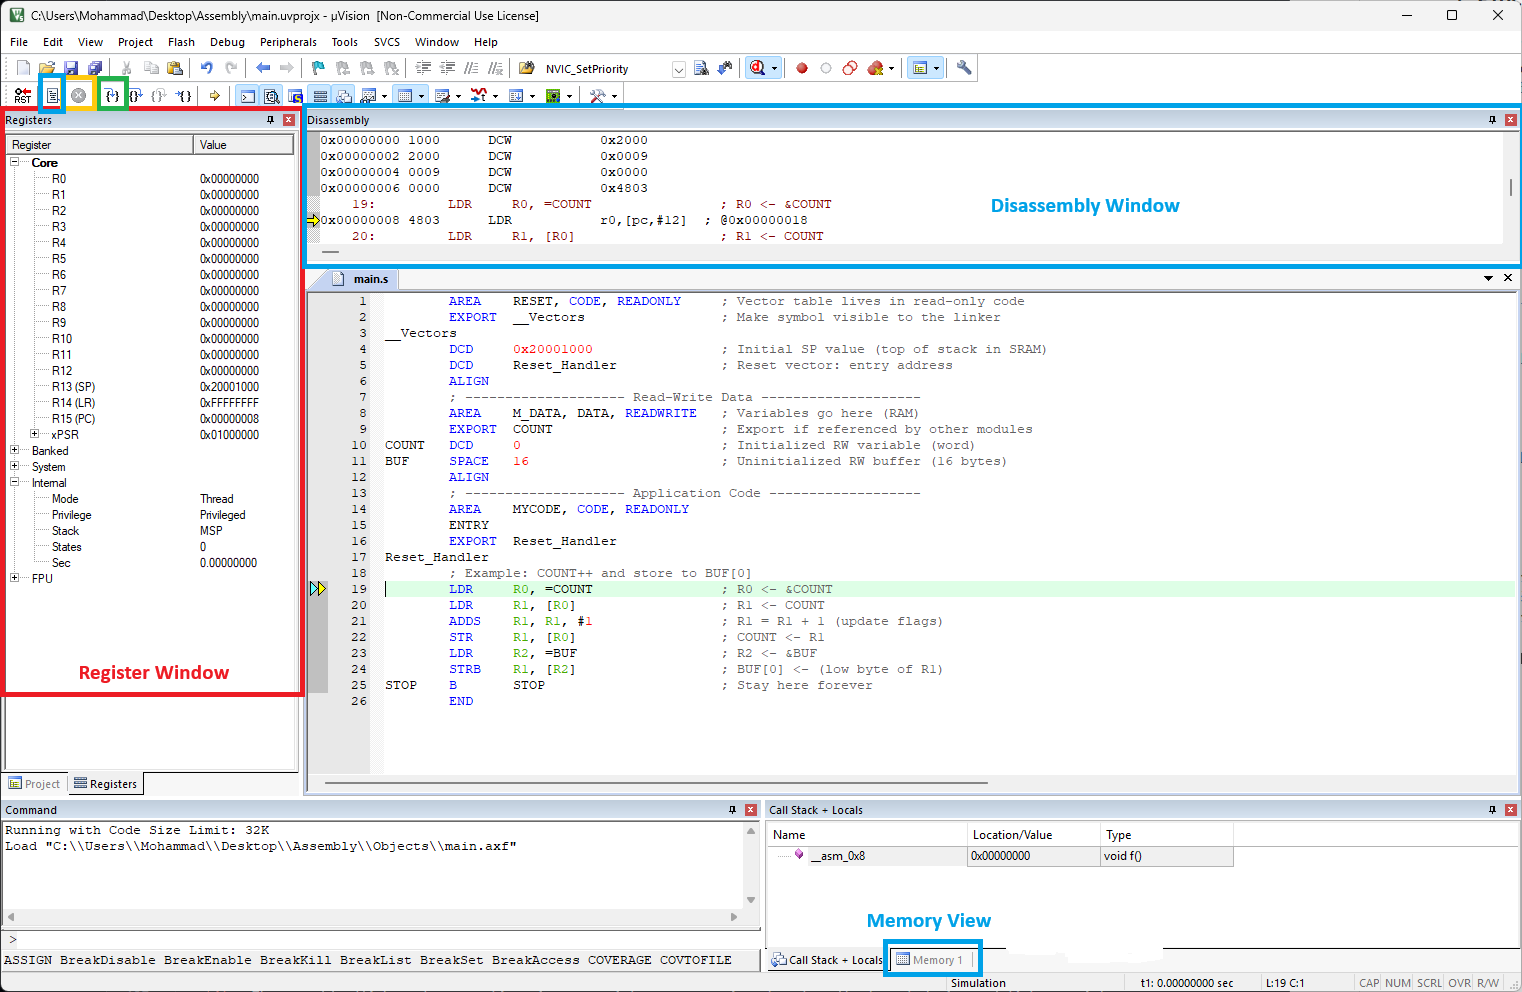
\includegraphics[width=\textwidth]{resources/keil_debug.png}
    \caption{Keil uVision5 Debugging Interface}
    \label{fig:keil_debug}
\end{figure}
Figure \ref{fig:keil_debug} shows the Keil uVision5 debugging interface. You can run and debug your assembly program using two main approaches:
\begin{enumerate}[nosep]
    \item \textbf{Step by Step Execution}:
    \begin{itemize}[nosep]
        \item Use the "Step" button (or press \texttt{F11}) marked in green in Figure \ref{fig:keil_debug} to execute your program one instruction at a time.
        \item Observe the changes in the registers and memory as you step through each instruction.
    \end{itemize}
    \item \textbf{Run the entire program}:
    \begin{itemize}[nosep]
        \item Use the "Run" button (or press \texttt{F5}) marked in blue in Figure \ref{fig:keil_debug} to execute your program continuously until it hits a breakpoint or completes execution.
        \item After running, you must stop the execution using the "Stop" button marked in yellow in Figure \ref{fig:keil_debug}.
        \item Check the final values in the registers and memory to verify the program's behavior.
    \end{itemize}
\end{enumerate}
\newpage
\subsection{Examples}
\subsubsection{Example 1: Simple Arithmetic Operations and Flag Manipulation}
The following example demonstrates basic arithmetic operations, flag manipulation, and conditional execution using ARM assembly language. It includes comments to guide you through each step.
\lstinputlisting[caption={Example 1: Simple Arithmetic Operations and Flag Manipulation}]{snippets/assembly/exp1/example1.asm}
\newpage
\subsubsection{Example 2: Using the Barrel Shifter and Conditional Execution}
The following example demonstrates the use of the barrel shifter for efficient data manipulation and conditional execution based on status flags. It includes comments to guide you through each step.
\lstinputlisting[caption={Example 2: Using the Barrel Shifter and Conditional Execution}]{snippets/assembly/exp1/example2.asm}


\chapter{ARM Cortex-M4 Instructions and Addressing Modes}

\section*{Learning Objectives}
\begin{itemize}[nosep]
  \item Recognize the three main categories of ARM Cortex-M4 instructions: data processing, load/store, and branch.  
  \item Perform arithmetic, logical, shift/rotate, and compare/test operations on registers.  
  \item Access memory using load and store instructions with different addressing modes (immediate, register offset, pre-/post-indexed).  
  \item Apply conditional execution using condition codes in the \texttt{xPSR}.  
  \item Observe and interpret the effects of instructions on registers, memory, and status flags using the \keil\ debugger.  
\end{itemize}

\section*{Experiment Overview}
This experiment introduces the core instruction set of the ARM Cortex-M4 processor.  
You will learn how to manipulate data in registers using arithmetic and logical instructions, how to transfer data between memory and registers using load/store instructions, and how to control program execution using condition codes and branches.  

In the process, you will:  
\begin{itemize}[nosep]
  \item Step through assembly instructions in the debugger and watch how registers and memory change.  
  \item Observe how flags (Z, N, C, V) are updated and used for conditional execution.  
  \item Practice pointer-style memory access through different addressing modes.  
\end{itemize}  

By the end of this lab, you will have gained practical experience in writing, executing, and debugging ARM Cortex-M4 assembly programs. These foundational skills in instruction-level programming, register manipulation, and memory access will serve as essential building blocks for subsequent experiments on flow control, interrupt handling, and peripheral interfacing.

\newpage
\tableofcontents
\newpage
\section{Theoretical Background}
As mentioned in Experiment 1, assembly instruction are split into three main categories: data processing, load/store, and branch instructions. This experiment focuses on data processing instructions, load/store instructions and their addressing modes. While branch instructions would be covered in more detail in Experiment 3 (Flow Control), a brief overview is provided here for completeness.
\subsection{Data Processing Instructions}
Data processing instructions perform arithmetic and logical operations on data stored in registers. They can also manipulate the condition flags in the xPSR based on the results of the operations. Common data processing instructions take the following form:
\[
\texttt{OPCODE\{<cond>\}\{S\} Rd, Rn, Operand2}
\]
where:
\begin{itemize}[nosep]
  \item \texttt{OPCODE}: the operation to be performed (e.g., \texttt{ADD}, \texttt{SUB}, \texttt{AND}, \texttt{ORR}).
  \item \texttt{<cond>}: optional condition code that predicates execution.
  \item \texttt{S}: optional suffix indicating whether to update the condition flags.
  \item \texttt{Rd}: destination register where the result is stored.
  \item \texttt{Rn}: first operand register.
  \item \texttt{Operand2}: second operand, which can be an immediate value limited to 8 bits, a register, or a barrel shifter operation.
\end{itemize}


\subsubsection{Arithmetic Instructions}
Arithmetic instructions perform basic mathematical operations. Some common arithmetic instructions include addition, subtraction, multiplication, and their variants. The following table summarizes some of the most commonly used arithmetic instructions in the ARM Cortex-M4 architecture.
\begin{table}[H]
\centering
\caption{Common ARM Cortex-M4 Arithmetic Instructions}
\small
\begin{tabularx}{\linewidth}{@{}l l l X@{}}
\toprule
\textbf{Instr.} & \textbf{Syntax} & \textbf{Operation} & \textbf{Description} \\
\midrule
ADD  & \texttt{ADD\{S\} Rd, Rn, Operand2}
     & $Rd \leftarrow Rn + Operand2$
     & \emph{Operand2} may be a register, an immediate, or a shifted register. \\
ADC  & \texttt{ADC\{S\} Rd, Rn, Operand2}
     & $Rd \leftarrow Rn + Operand2 + C$
     & Adds carry-in $C$. \\
SUB  & \texttt{SUB\{S\} Rd, Rn, Operand2}
     & $Rd \leftarrow Rn - Operand2$
     & Standard subtraction. \\
SBC  & \texttt{SBC\{S\} Rd, Rn, Operand2}
     & $Rd \leftarrow Rn - Operand2 - (1 - C)$
     & Subtract with borrow (borrow encoded via carry flag $C$). \\
RSB  & \texttt{RSB\{S\} Rd, Rn, Operand2}
     & $Rd \leftarrow Operand2 - Rn$
     & Reverse subtract. \\
MUL  & \texttt{MUL\{S\} Rd, Rn, Rm}
     & $Rd \leftarrow (Rn \times Rm)_{[31{:}0]}$
     & 32$\times$32 $\rightarrow$ low 32 bits. \\
MLA  & \texttt{MLA Rd, Rn, Rm, Ra}
     & $Rd \leftarrow (Rn \times Rm) + Ra$
     & Multiply-accumulate. \\
MLS  & \texttt{MLS Rd, Rn, Rm, Ra}
     & $Rd \leftarrow Ra - (Rn \times Rm)$
     & Multiply-subtract. \\
UMULL & \texttt{UMULL RdLo, RdHi, Rn, Rm}
      & $\{RdHi,RdLo\} \leftarrow Rn \times Rm$
      & Unsigned 32$\times$32 $\rightarrow$ 64-bit product. \\
SMULL & \texttt{SMULL RdLo, RdHi, Rn, Rm}
      & $\{RdHi,RdLo\} \leftarrow Rn \times Rm$
      & Signed 32$\times$32 $\rightarrow$ 64-bit product. \\
\bottomrule
\end{tabularx}

\vspace{2pt}
\footnotesize\emph{Note:} $C$ denotes the carry flag in \texttt{xPSR}. \emph{Operand2} may be an immediate or a shifted register depending on the encoding.
\end{table}
\subsubsection{Logical and Move Instructions}
Logical instructions perform bitwise operations on data, while move instructions transfer data between registers or load immediate values. The following table summarizes some of the most commonly used logical and move instructions in the ARM Cortex-M4 architecture.
\begin{table}[H]
\centering
\caption{Logical and Move Instructions}
\small
\begin{tabularx}{\linewidth}{@{}l l l X@{}}
\toprule
\textbf{Instr.} & \textbf{Syntax} & \textbf{Operation} & \textbf{Description} \\
\midrule
AND  & \texttt{AND Rd, Rn, Operand2} & $Rd \leftarrow Rn \,\&\, Operand2$ & Bitwise AND. \\
ORR  & \texttt{ORR Rd, Rn, Operand2} & $Rd \leftarrow Rn \,|\, Operand2$ & Bitwise OR. \\
EOR  & \texttt{EOR Rd, Rn, Operand2} & $Rd \leftarrow Rn \oplus Operand2$ & Bitwise XOR. \\
BIC  & \texttt{BIC Rd, Rn, Operand2} & $Rd \leftarrow Rn \,\&\, \neg Operand2$ & Bit clear. \\
MVN  & \texttt{MVN Rd, Operand2}     & $Rd \leftarrow \neg Operand2$ & Bitwise NOT of operand. \\
MOV  & \texttt{MOV Rd, Operand2}     & $Rd \leftarrow Operand2$ & Register or immediate move. \\
MOVW & \texttt{MOVW Rd, \#imm16}     & $Rd[15{:}0] \leftarrow imm16$ & Write low halfword. \\
MOVT & \texttt{MOVT Rd, \#imm16}     & $Rd[31{:}16] \leftarrow imm16$ & Write high halfword (low preserved). \\
\bottomrule
\end{tabularx}

\vspace{2pt}
\footnotesize\emph{Note:} $C$ denotes the carry flag in \texttt{xPSR}. \emph{Operand2} may be an immediate or a shifted register depending on the encoding.
\end{table}
We will be using bitwise logical instructions extensively in this experiment to manipulate specific bits in registers from setting, clearing, and flipping certain bits, or checking if certain bits are set or cleared.
\subsubsection*{Setting and Clearing Bits}
To set, clear, or toggle specific bits in a register, you can use the following logical instructions:
\begin{itemize}[nosep]
    \item \texttt{ORR Rd, Rn, \#mask}: Sets bits in \texttt{Rd} where the corresponding bits in \texttt{mask} are 1.
    \item \texttt{BIC Rd, Rn, \#mask}: Clears bits in \texttt{Rd} where the corresponding bits in \texttt{mask} are 1.
    \item \texttt{EOR Rd, Rn, \#mask}: Toggles bits in \texttt{Rd} where the corresponding bits in \texttt{mask} are 1.
\end{itemize}
to check if certain bits are set or cleared, you can use the \texttt{TST} instruction:
\begin{itemize}[nosep]
    \item \texttt{TST Rn, \#mask}: Performs a bitwise AND between \texttt{Rn} and \texttt{mask}, updating the condition flags based on the result. If the result is zero, the zero flag (Z) is set, indicating that none of the bits in \texttt{mask} are set in \texttt{Rn}.
\end{itemize}

\subsubsection{Shift and Rotate Instructions}
\begin{table}[H]
\centering
\caption{Shift and Rotate Instructions}
\small
\begin{tabularx}{\linewidth}{@{}l l l X@{}}
\toprule
\textbf{Instr.} & \textbf{Syntax} & \textbf{Operation} & \textbf{Description} \\
\midrule
LSL & \texttt{LSL Rd, Rm, \#sh\textbar Rs}
    & $Rd \leftarrow Rm \ll sh$
    & Logical left shift by immediate or by register. \\
LSR & \texttt{LSR Rd, Rm, \#sh\textbar Rs}
    & $Rd \leftarrow Rm \gg sh$
    & Logical right shift (zero fill). \\
ASR & \texttt{ASR Rd, Rm, \#sh\textbar Rs}
    & $Rd \leftarrow Rm \gg sh$
    & Arithmetic right shift (sign fill). \\
ROR & \texttt{ROR Rd, Rm, \#sh\textbar Rs}
    & $Rd \leftarrow \mathrm{ROR}(Rm, sh)$
    & Rotate right by immediate or by register. \\
RRX & \texttt{RRX Rd, Rm}
    & $Rd \leftarrow \mathrm{ROR}_{C}(Rm, 1)$
    & Rotate right 1 bit through carry (uses $C$ as incoming bit 31, outgoing bit 0 $\rightarrow C$). \\
\bottomrule
\end{tabularx}

\vspace{2pt}
\footnotesize\emph{Note:} Shift amount can be an immediate \texttt{\#sh} (0--31) or a register \texttt{Rs} (low 8 bits used). 
For immediates: \texttt{LSL \#0} = no shift; \texttt{LSR \#0} is treated as shift by 32; \texttt{ASR \#0} is treated as shift by 32; \texttt{ROR \#0} means \texttt{RRX}.
\end{table}
Not all shift/rotate instructions are explicitly present in the ARMv7-M ISA. For example, there is no ROL (rotate left) or ASL (arithmetic shift left) instruction, as these operations can be achieved using existing shift instructions: ROL can be implemented using ROR with a complementary shift amount, and ASL is equivalent to LSL.
\subsubsection{Compare and Test Instructions}
Compare and test instructions are used to compare values and set condition flags without producing a direct result in a register. These instructions are useful for conditional execution and branching based on the results of comparisons. The following table summarizes the compare and test instructions in the ARM Cortex-M4 architecture.
\begin{table}[H]
\centering
\caption{Compare and Test Instructions}
\small
\begin{tabularx}{\linewidth}{@{}l l l X@{}}
\toprule
\textbf{Instr.} & \textbf{Syntax} & \textbf{Operation} & \textbf{Description} \\
\midrule
CMP & \texttt{CMP Rn, Operand2} & Flags from $(Rn - Operand2)$ & Comparison; no register result. \\
CMN & \texttt{CMN Rn, Operand2} & Flags from $(Rn + Operand2)$ & “Compare negative” (add then set flags). \\
TST & \texttt{TST Rn, Operand2} & Flags from $(Rn \,\&\, Operand2)$ & Bitwise test; no register result. \\
TEQ & \texttt{TEQ Rn, Operand2} & Flags from $(Rn \oplus Operand2)$ & XOR test; no register result. \\
\bottomrule
\end{tabularx}
\end{table}

\subsection{Load and Store Instructions}
Since the ARM Cortex-M4 architecture follows the RISC design philosophy, it uses a load/store architecture. This means that data processing instructions can only operate on data in registers, and any data in memory must first be loaded into a register before it can be processed. Similarly, results from data processing operations must be stored back to memory if they need to be preserved. The following table summarizes the load and store instructions in the ARM Cortex-M4 architecture.

\begin{table}[H]
\centering
\caption{Load and Store Instructions (Summary)}
\small
\begin{tabularx}{\linewidth}{@{}l l X@{}}
\toprule
\textbf{Instr.} & \textbf{Syntax Example} & \textbf{Description} \\
\midrule
LDR / STR       & \texttt{LDR/STR Rt, [Rn, \#off]} & Load/store a 32-bit word. \\
LDRB / STRB     & \texttt{LDRB/STRB Rt, [Rn, \#off]} & Load/store an 8-bit byte. \\
LDRH / STRH     & \texttt{LDRH/STRH Rt, [Rn, \#off]} & Load/store a 16-bit halfword. \\
LDRSB / LDRSH   & \texttt{LDRSB/LDRSH Rt, [Rn, \#off]} & Load signed byte/halfword and sign-extend to 32 bits. \\
LDRD / STRD     & \texttt{LDRD/STRD Rt, Rt2, [Rn, \#off]} & Load/store a 64-bit doubleword (two registers). \\
\bottomrule
\end{tabularx}
\vspace{2pt}
\end{table}

\begin{itemize}[nosep]
  \item \texttt{LDR Rt, =label} is a \emph{pseudo-instruction}. The assembler replaces it with code to load the \textbf{address} of \texttt{label} into \texttt{Rt}.
  \item \texttt{LDR Rt, label} (without \texttt{=}) loads the \textbf{contents stored at} \texttt{label}.
\end{itemize}
\newpage
\begin{lstlisting}[caption={Examples of Load and Store Instructions}]
        AREA    MYDATA, DATA, READONLY
XVAL    DCD     0x12345678        ; word in memory
YPTR    DCD     YVAL              ; contains the address of YVAL

        AREA    MYDATA2, DATA, READWRITE
YVAL    DCD     0

        AREA    MYCODE, CODE, READONLY
        ENTRY
        EXPORT  Reset_Handler

Reset_Handler
        LDR     R0, =XVAL         ; R0 = &XVAL (address of XVAL)
        LDR     R1, [R0]          ; R1 = 0x12345678 (load word from memory)

        LDRB    R2, [R0]          ; R2 = 0x78 (lowest byte of XVAL)
        LDRH    R3, [R0]          ; R3 = 0x5678 (lowest halfword of XVAL)

        MOV     R4, #0xFF
        LDR     R0, YPTR          ; R0 = contents of YPTR = &YVAL
        STRB    R4, [R0]          ; store 0xFF into YVAL (low byte only)

STOP    B       STOP
        END
\end{lstlisting}
\noindent\textit{Note:}  
\begin{itemize}[nosep]
    \item The line \texttt{YPTR DCD YVAL} allocates a 32-bit word at the label \texttt{YPTR} and initializes it with the address of \texttt{YVAL}.  
    \item Executing \texttt{LDR R0, YPTR} loads the contents of \texttt{YPTR} (the address of \texttt{YVAL}) into \texttt{R0}, making \texttt{R0} a pointer to \texttt{YVAL}.  
    \item By contrast, \texttt{LDR R0, =YVAL} directly loads the address of \texttt{YVAL} into \texttt{R0} without going through memory.  
\end{itemize}

\begin{center}
\begin{tabular}{|c|c|c|}
\hline
Address & Label & Contents \\
\hline
0x2000 & XVAL & 0x12345678 \\
0x2004 & YPTR & 0x2008 (address of YVAL) \\
0x2008 & YVAL & 0x00000000 \\
\hline
\end{tabular}
\end{center}

\subsection{Branch Instructions and Condition Codes}
Branch instructions change the flow of execution by jumping to a different part of the program. They can be unconditional or conditional based on the status flags in the xPSR. The following table summarizes the branch instructions in the ARM Cortex-M4 architecture.
\begin{table}[H]
\centering
\caption{Branch Instructions}
\small
\begin{tabularx}{\linewidth}{@{}l l X@{}}
\toprule
\textbf{Instr.} & \textbf{Syntax Example} & \textbf{Description} \\
\midrule
B    & \texttt{B label} & Unconditional branch to \texttt{label}. \\
B<cond> & \texttt{B<cond> label} & Conditional branch based on condition flags. \\
BL   & \texttt{BL label} & Branch with link (calls subroutine, saves return address in LR). \\
BX   & \texttt{BX Rm} & Branch to address in register \texttt{Rm} (LR is usually used here). \\
\bottomrule
\end{tabularx}
\vspace{2pt}
\end{table}

\begin{table}[H]
\centering
\caption{Condition Codes}
\small
\begin{tabularx}{\linewidth}{@{}l l X@{}}
\toprule
\textbf{Cond.} & \textbf{Meaning} & \textbf{Description} \\
\midrule
EQ  & Equal          & Z set (zero result) \\
NE  & Not equal      & Z clear (non-zero result) \\
CS/HS & Carry set / Unsigned higher or same & C set \\
CC/LO & Carry clear / Unsigned lower & C clear \\
MI  & Minus / Negative & N set (negative result) \\
PL  & Plus / Positive or zero & N clear \\
VS  & Overflow set   & V set \\
VC  & Overflow clear & V clear \\
HI  & Unsigned higher & C set and Z clear \\
LS  & Unsigned lower or same & C clear or Z set \\
GE  & Signed greater than or equal & N == V \\
LT  & Signed less than & N != V \\
GT  & Signed greater than & Z clear and N == V \\
LE  & Signed less than or equal & Z set or N != V \\
AL  & Always         & (unconditional) \\
NV  & Never          & (not used) \\
\bottomrule
\end{tabularx}
\vspace{2pt}
\end{table}
\subsection{Addressing Modes}

Addressing modes define how the effective address or operand value is obtained by an instruction. 
The ARM Cortex-M4 supports several common addressing modes, summarized below:

\begin{table}[H]
\centering
\caption{General Addressing Modes in ARM Cortex-M4}
\small
\begin{tabularx}{\linewidth}{@{}l l X@{}}
\toprule
\textbf{Mode} & \textbf{Syntax Example} & \textbf{Description} \\
\midrule
Immediate      & \texttt{MOV R0, \#10}          & Operand is a constant value encoded in the instruction. \\
Register Direct& \texttt{MOV R0, R1}            & Operand is taken directly from a register. \\
Register Indirect & \texttt{LDR R0, [R1]}       & Register holds the address of the operand in memory. \\
Register Offset & \texttt{LDR R0, [R1, R2]}     & Effective address = base register + offset register. \\
Immediate Offset & \texttt{LDR R0, [R1, \#4]}   & Effective address = base register + constant offset. \\
Pre-indexed    & \texttt{LDR R0, [R1, \#4]!}    & Base updated first, then memory access. \\
Post-indexed   & \texttt{LDR R0, [R1], \#4}     & Memory access first, then base register updated. \\
\bottomrule
\end{tabularx}
\vspace{2pt}
\end{table}
\newpage
\begin{lstlisting}[caption={Examples of Offset, Pre-indexed, and Post-indexed Addressing Modes}]
; Immediate Offset
    LDR     R0, [R1, #4]     ; R0 = word at memory[R1 + 4]
; Register Offset
    LDR     R0, [R1, R2]    ; R0 = word at memory[R1 + R2]
; Pre-indexed
    LDR     R0, [R1, #4]!    ; R1 = R1 + 4, then load R0 = [R1]
; Post-indexed
    LDR     R0, [R1], #4     ; load R0 = [R1], then R1 = R1 + 4
\end{lstlisting}

\newpage
\section{Procedure}

\subsection{Examples}

\subsubsection{Example 1 --- Arithmetic and Bitwise Operations}
This example demonstrates basic arithmetic and bitwise operations in ARM assembly, showing how to set, clear, and flip bits.

\lstinputlisting[caption={Arithmetic and bitwise operations example}]{snippets/assembly/exp2/example1.asm}
\newpage
\subsubsection{Example 2 --- Status Flags and Logical Tests}
This example demonstrates the use of status flags and logical tests in ARM assembly, including conditional execution based on comparison results.

\lstinputlisting[caption={Status flags and logical tests example}]{snippets/assembly/exp2/example2.asm}
\newpage
\subsubsection{Example 3 --- Load/Store with Different Addressing Modes}
This example demonstrates load and store instructions using various addressing modes.
\lstinputlisting[caption={Load/store with different addressing modes example}]{snippets/assembly/exp2/example3.asm}
\subsection{Tasks}

\subsubsection{Task 1 --- Bitwise Register Manipulation}
Start with \texttt{R0 = 0x12345678}. Perform the following operations and observe the results in the debugger:
\begin{itemize}[nosep]
    \item Clear bits 4--7 (second hex nibble).
    \item Set bits 8--11 (force nibble to \texttt{F}).
    \item Toggle bits 28--31 (highest nibble).
\end{itemize}
\emph{Hint:} Use \texttt{BIC}, \texttt{ORR}, and \texttt{EOR} with appropriate masks.

\subsubsection{Task 2 --- Arithmetic and Status Flags}
Assume initial values \texttt{R0 = 25} and \texttt{R1 = 10}.
\begin{itemize}[nosep]
    \item Add \texttt{R0 + R1}, store the result in \texttt{R2}.
    \item Subtract \texttt{R1} from \texttt{R0}, store the result in \texttt{R3}.
    \item Multiply \texttt{R0} and \texttt{R1}, store the result in \texttt{R4}.
    \item Compare \texttt{R0} and \texttt{R1} using \texttt{CMP}.
          If greater, set \texttt{R5 = 1}; otherwise, set \texttt{R5 = 0}.
\end{itemize}
Observe how the \texttt{Z} (zero) and \texttt{N} (negative) flags in the xPSR are affected.

\subsubsection{Task 3 --- Addressing Modes with an Array}
Given the following array:
\begin{lstlisting}
ARRAY   DCD  0x11, 0x22, 0x33, 0x44
\end{lstlisting}

Perform the following loads using different addressing modes:
\begin{itemize}[nosep]
    \item Load the first element (\texttt{0x11}) using \emph{immediate offset}.
    \item Load the second element (\texttt{0x22}) using \emph{pre-indexed} addressing.
    \item Load the third element (\texttt{0x33}) using \emph{post-indexed} addressing.
    \item Load the fourth element (\texttt{0x44}) using a \emph{register offset} (offset in another register).
\end{itemize}

Store each result into an output buffer \texttt{OUT} and verify the results in memory.


\chapter{Flow Control, Procedures, and Stack Management}

\section*{Learning Objectives}
After completing this experiment, you will be able to:
\begin{itemize}[nosep]
  \item Implement conditional and unconditional branching using ARM branch instructions.
  \item Design and implement loop constructs (\texttt{for}, \texttt{while}) using compare and branch instructions.
  \item Create and call procedures with proper parameter passing and return mechanisms.
  \item Manage the stack for local variables, parameter passing, and nested procedure calls.
  \item Apply the ARM Procedure Call Standard (AAPCS) to ensure correct register usage and calling conventions.
\end{itemize}

\section*{Experiment Overview}
This experiment introduces program control flow, procedure implementation, and stack management on the ARM Cortex-M4 processor. 
You will learn how to control program execution using branches and loops, create modular and reusable code using procedures, and manage memory efficiently through stack operations.

\noindent In this experiment, you will:
\begin{itemize}[nosep]
  \item Implement conditional branches and loop structures at the assembly level.
  \item Write and call procedures that follow standard calling conventions.
  \item Handle nested calls and parameter passing using the stack.
  \item Observe and analyze how the stack changes during procedure entry and return.
\end{itemize}

By the end of this lab, you will understand how to use branching and looping for program control, write well-structured procedures that follow AAPCS rules, and manage the stack during function calls and nested procedures.

\newpage
\etocsetnexttocdepth{subsubsection}
\localtableofcontents
\bigskip
\newpage
\section{Theoretical Background}
\subsection{Flow Control}
Flow control instructions alter the sequential execution of instructions by changing the program counter (PC). These instructions enable the implementation of conditional statements, loops, and procedure calls that are fundamental to structured programming.

\subsubsection{Condition Evaluation}
Before implementing control flow, we must understand how to evaluate conditions and set processor flags. ARM provides dedicated instructions for comparing values and testing bit patterns that update the condition flags without storing results.

\begin{table}[H]
\centering
\caption{ARM Cortex-M4 Compare and Test Instructions}
\small
\begin{tabularx}{\linewidth}{@{}l l X@{}}
\toprule
\textbf{Instr.} & \textbf{Syntax} & \textbf{Description / Usage} \\
\midrule
CMP     & \texttt{CMP Rn, Operand2}   & Compare \texttt{Rn} with \texttt{Operand2} (\texttt{Rn - Operand2}); updates flags (Z, N, C, V). \\
CMN     & \texttt{CMN Rn, Operand2}   & Compare negative (\texttt{Rn + Operand2}); used for checking against negative values. \\
TST     & \texttt{TST Rn, Operand2}   & Logical AND test (\texttt{Rn AND Operand2}); sets Z if all tested bits are 0. \\
TEQ     & \texttt{TEQ Rn, Operand2}   & Logical XOR test (\texttt{Rn EOR Operand2}); sets Z if operands are equal. \\
\bottomrule
\end{tabularx}
\end{table}

\paragraph{Usage Notes:}
\begin{itemize}[nosep]
  \item These instructions only affect the condition flags (N, Z, C, V) — they do not store a result.
  \item \texttt{CMP}/\texttt{CMN} are arithmetic comparisons; \texttt{TST}/\texttt{TEQ} are logical bitwise comparisons.
  \item Many data-processing instructions can update flags by appending \texttt{S} (e.g., \texttt{ADDS}, \texttt{SUBS}).
  \item Common use: immediately followed by conditional branches such as \texttt{BEQ}, \texttt{BNE}, \texttt{BGT}, etc.
\end{itemize}

\noindent\paragraph{Examples:}
\hfill
\begin{lstlisting}[caption={Arithmetic comparison using CMP}]
    CMP     R0, #10          ; Compare R0 with 10
    BLT     LessThan10       ; Branch if R0 < 10
    BGE     GreaterOrEqual   ; Otherwise, R0 >= 10
\end{lstlisting}

\begin{lstlisting}[caption={Bit test using TST}]
    MOV     R1, #0x12        ; R1 = 0001 0010b
    TST     R1, #0x10        ; Test if bit 4 is set
    BEQ     BitClear         ; Branch if bit 4 = 0 (Z=1)
    BNE     BitSet           ; Branch if bit 4 = 1 (Z=0)
\end{lstlisting}

\begin{lstlisting}[caption={Equality check using TEQ}]
    MOV     R2, #0x55
    MOV     R3, #0x55
    TEQ     R2, R3           ; XOR -> result 0, sets Z=1
    BEQ     ValuesEqual      ; Branch if equal
\end{lstlisting}

\subsubsection{Conditional Branching}
Branch instructions are the primary mechanism for implementing flow control in ARM assembly. They modify the program counter to jump to different parts of the code based on conditions or unconditionally.

\begin{table}[H]
\centering
\caption{ARM Cortex-M4 Branch Instructions}
\small
\begin{tabularx}{\linewidth}{@{}l l X@{}}
\toprule
\textbf{Instr.} & \textbf{Syntax} & \textbf{Description / Usage} \\
\midrule
B       & \texttt{B label}        & Unconditional branch to \texttt{label} (always jumps) \\
B\texttt{<cond>} & \texttt{B<cond> label}  & Conditional branch based on flags \\
BL      & \texttt{BL label}       & Branch with link: calls a subroutine, storing return address in \texttt{LR}. \\
BX      & \texttt{BX Rm}          & Branch to address in register, often \texttt{BX LR} to return from a subroutine. \\
CBZ     & \texttt{CBZ Rn, label}  & Branch if \texttt{Rn == 0}. Example: \texttt{CBZ R0, Done}. \\
CBNZ    & \texttt{CBNZ Rn, label} & Branch if \texttt{Rn != 0}. Example: loop until counter reaches zero. \\
\bottomrule
\end{tabularx}
\end{table}

\paragraph{\texttt{CBZ/CBNZ}} instructions have specific constraints:
\begin{itemize}[nosep]
  \item \textbf{Register}: operand must be a low register \texttt{R0--R7}.
  \item \textbf{Range}: branch is \emph{forward-only}; the destination must be within 0--126 bytes after the instruction.
  \item \textbf{Flags}: does not update condition flags (\texttt{N, Z, C, V}).
\end{itemize}
For backward or longer jumps, use \texttt{CMP}/\texttt{TST} with conditional branches (\texttt{BEQ}, \texttt{BNE}, \texttt{BGT}, \dots).

\subsubsection{Conditional Execution}
ARM assembly supports conditional execution, where most instructions can be conditionally executed based on the current state of the condition flags. This feature allows for efficient implementation of conditional statements without explicit branching.

\paragraph{Conditional Instruction Format:}
Most ARM instructions can be made conditional by appending a condition code suffix:
\[
\texttt{OPCODE\{<cond>\} Rd, Rn, Operand2}
\]

\paragraph{Examples:}
\begin{itemize}[nosep]
    \item \texttt{ADDEQ R0, R1, R2} — Add only if equal (Z=1)
    \item \texttt{MOVNE R3, \#10} — Move only if not equal (Z=0)
    \item \texttt{SUBGT R4, R4, \#1} — Subtract only if greater than (signed)
\end{itemize}

\paragraph{Advantages of Conditional Execution:}
\begin{itemize}[nosep]
    \item \textbf{Performance}: Eliminates branch instructions for simple conditional operations
    \item \textbf{Code density}: Reduces the number of instructions needed
    \item \textbf{Pipeline efficiency}: Avoids branch prediction penalties for simple conditions
    \item \textbf{Atomic operations}: Multiple related conditional operations can be grouped
\end{itemize}
\subsubsection{How Branch Instructions Work}

Branch instructions change the flow of execution by modifying the Program Counter (\texttt{PC}). 
When a branch is executed, the instruction encodes an \emph{offset} which is added to the current value of the \texttt{PC}.

\paragraph{Offset calculation:}  
The branch instruction contains a signed immediate value (positive or negative).  
The processor adds this offset (aligned to halfword boundaries) to the current \texttt{PC}.  
\begin{itemize}
    \item A \emph{positive offset} causes a \textbf{forward branch} (jump to a higher memory address, later in the program).  
    \item A \emph{negative offset} causes a \textbf{backward branch} (jump to a lower memory address, earlier in the program).  
\end{itemize} 

\paragraph{Example:}  
Suppose a branch instruction is located at address \texttt{0x100}, and the assembler encodes an immediate offset of \texttt{-0x08}.  
The effective target address will be:
\[
0x100 + 4 + (-0x08) = 0xFC
\]
This means the processor jumps \textbf{backward} to an earlier instruction.  
Such negative offsets are typically used to implement loops (e.g., repeat until zero).

\subsubsection{Condition Codes}
Conditional branches use condition codes that test the processor status flags (N, Z, C, V) set by previous instructions. These enable implementing high-level constructs like if-statements and loops.

\begin{table}[H]
\centering
\caption{Common ARM Condition Codes}
\small
\begin{tabularx}{0.72\linewidth}{@{}l l X@{}}
\toprule
\textbf{Cond.} & \textbf{Meaning} & \textbf{Description} \\
\midrule
EQ  & Equal                     & Execute if $Z=1$. \\
NE  & Not equal                 & Execute if $Z=0$. \\
CS/HS & Carry set / Unsigned higher or same & Execute if $C=1$. \\
CC/LO & Carry clear / Unsigned lower        & Execute if $C=0$. \\
MI  & Minus (negative)          & Execute if $N=1$. \\
PL  & Plus (non-negative)       & Execute if $N=0$. \\
VS  & Overflow set              & Execute if $V=1$. \\
VC  & Overflow clear            & Execute if $V=0$. \\
HI  & Unsigned higher           & Execute if $C=1$ \emph{and} $Z=0$. \\
LS  & Unsigned lower or same    & Execute if $C=0$ \emph{or} $Z=1$. \\
GE  & Greater or equal (signed) & Execute if $N=V$. \\
LT  & Less than (signed)        & Execute if $N\neq V$. \\
GT  & Greater than (signed)     & Execute if $Z=0$ \emph{and} $N=V$. \\
LE  & Less or equal (signed)    & Execute if $Z=1$ \emph{or} $N\neq V$. \\
AL  & Always                    & Always execute (default if no condition). \\
NV  & Never                     & Reserved / do not use. \\
\bottomrule
\end{tabularx}
\end{table}

\subsection{Loop Patterns}
Loops are fundamental control structures that repeat a block of code based on conditions. ARM assembly implements loops using combinations of compare instructions, conditional branches, and counters.

\subsubsection{For Loop Structure}
A typical for loop has the structure: initialization, condition check, body execution, and increment/decrement. This type of loop executes a known number of times.
\begin{lstlisting}[caption={Declaring Array and Length}]
        AREA M_DATA, DATA, READONLY
array   DCD 10, 20, 30, 40, 50   ; array of 5 integers
length  EQU 5                    ; number of elements (; just a constant, no memory)
\end{lstlisting}
\begin{lstlisting}[caption={For loop implementation pattern}]
        ; Initialization
        MOV     R0, #0                  ; i = 0
        MOV     R1, #0                  ; sum = 0
        LDR     R3, =array              ; load base address of array into R3

for_start
        ; Condition check
        CMP     R0, #length             ; compare i with length
        BGE     for_end                 ; if i >= length, exit loop

        ; Loop body
        LDR     R2, [R3, R0, LSL #2]    ; load array[i]; EA: R3 + (R0 * 4)
        ADD     R1, R1, R2              ; sum += array[i]

        ; Increment
        ADD     R0, R0, #1              ; i++
        B       for_start               ; repeat

for_end
\end{lstlisting}
\subsubsection{While Loop Structure}
While loops check the condition before executing the loop body, potentially executing zero times if the initial condition is false. This type of loop is useful when the number of iterations is not known in advance and depends on dynamic conditions.
\begin{lstlisting}[caption={Declaring Null-Terminated String}]
        AREA M_DATA, DATA, READONLY
mystring DCB "Hello World!", 0    ; null-terminated string
\end{lstlisting}
\paragraph{Note:} \texttt{0} and \texttt{'0'} are two different values, as the former is actually zero, while the latter is the ASCII code for the character '0' (which is 48 in decimal).
\newpage

\begin{lstlisting}[caption={While loop with string processing example}]
    ; Intialization
    LDR     R0, =mystring   ; pointer to string
    MOV     R1, #0          ; character count = 0

while_start
                            ; Condition check
    LDRB    R2, [R0], #1    ; load current character and post-increment pointer
    CMP     R2, #0          ; check for null terminator
    BEQ     while_end       ; if zero, exit loop
    
                            ; Loop body - do something with R2

    
    B       while_start     ; repeat
while_end
\end{lstlisting}


\subsection{Procedures and Stack}

\subsubsection{ARM Architecture Procedure Call Standard (AAPCS)}

Procedures are reusable blocks of code that encapsulate a specific task. They promote modular design, code reuse, and clearer program structure. In ARM assembly, procedures are implemented using branch-and-link instructions along with register usage conventions defined by the ARM Architecture Procedure Call Standard (AAPCS).

The AAPCS is the set of rules that define how functions exchange data and how registers must be preserved during a procedure call:

\begin{itemize}[nosep]
  \item \textbf{R0--R3}: Hold the first four parameters. \texttt{R0} also holds the return value. Caller-saved.
  \item \textbf{Stack}: Any additional parameters beyond the first four are passed on the stack.
  \item \textbf{R4--R11}: Must be preserved by the callee. If a procedure uses them, it must save and restore them. 
  \item \textbf{SP (R13)}: Stack pointer, always points to the current top of the stack.
  \item \textbf{LR (R14)}: Link register holds the return address. Caller-saved.
\end{itemize}
\paragraph{Note:} Callees are the procedures being called, while callers are the ones calling the procedure.

\subsubsection{Procedure Templates}

A procedure is entered with a \texttt{BL} (branch-with-link) instruction, which stores the return address in the link register \texttt{LR}. The callee returns by branching to \texttt{LR} (e.g., \texttt{BX LR}). By the AAPCS, the first four arguments are passed in \texttt{R0--R3} and the primary return value is placed in \texttt{R0}.
\newpage
\paragraph{Basic Procedure Template}

\paragraph{Example:} simple procedure that expects two integers in \texttt{R0} and \texttt{R1} and returns their sum in \texttt{R0}.

\begin{lstlisting}[caption={Basic procedure structure}]
AddTwo  PROC
        ADD R0, R0, R1   ; return R0+R1 in R0
        BX  LR
        ENDP
\end{lstlisting}
\paragraph{Note:} The \texttt{PROC} and \texttt{ENDP} directives help define the start and end of a procedure and they could be safely omitted.

\paragraph{Procedure with Preserved Registers}

When a procedure uses callee-saved registers (R4-R11), it must preserve their original values by saving them on the stack and restoring them before returning:

\begin{lstlisting}[caption={Procedure using preserved registers}]
ProcessArray PROC
        PUSH    {R4-R6, LR}     ; Save used registers and LR
        MOV     R4, R0          ; Save array pointer
        MOV     R5, R1          ; Save array length  
        MOV     R6, #0          ; Initialize counter
        
        ; Process array using R4, R5, R6...
        
        MOV     R0, R6          ; Return counter value
        POP     {R4-R6, PC}     ; Restore registers and return
        ENDP
\end{lstlisting}

\paragraph{Nested Procedure Calls}

When one procedure calls another, the link register (\texttt{LR}) must be preserved, otherwise the return address would be lost. This is done by pushing \texttt{LR} onto the stack before making another call.

\begin{lstlisting}[caption={Nested procedure example}]
OuterProc
        PUSH    {LR}            ; Save return address
        BL      InnerProc       ; Call inner procedure
        MOV     R1, R0          ; Use return value
        POP     {PC}            ; Return to caller

InnerProc 
        MOV     R0, #42         ; Return value
        BX      LR              ; Return
\end{lstlisting}


\subsubsection{Stack Model (Full, Descending)}
There are four common stack models based on two characteristics: whether the stack is full or empty, and whether it grows up (ascending) or down (descending). 
\begin{itemize}[nosep]
    \item \textbf{Full Ascending}: SP points to the last used location; stack grows toward higher addresses.
    \item \textbf{Empty Ascending}: SP points to the next free location; stack grows toward higher addresses.
    \item \textbf{Empty Descending}: SP points to the next free location; stack grows toward lower addresses.
    \item \textbf{Full Descending}: SP points to the last used location; stack grows toward lower addresses.
\end{itemize}
The ARM Cortex-M4 uses a \textbf{full descending stack}, meaning:
\begin{itemize}[nosep]
    \item The stack pointer (\texttt{SP}) points to the last used location (full).
    \item The stack grows toward lower memory addresses (descending).
\end{itemize}
\subsubsection{Stack Operations}

The Cortex-M4 provides \texttt{PUSH} and \texttt{POP} instructions that automatically update the stack pointer (\texttt{SP}) and allow saving or restoring multiple registers in a single instruction.  
These operations are essential for implementing procedure calls, local variables, and context switching.
\paragraph{PUSH}

The \texttt{PUSH} instruction saves one or more registers onto the stack in a single operation.
When executed, the stack pointer (\texttt{SP}) is decremented to reserve space, and the specified registers are written to consecutive memory locations starting from the new \texttt{SP} value.
\textbf{Rule:} \texttt{PUSH} stores registers on the stack, with the \textbf{lowest-numbered register} placed at the \textbf{lowest memory address} and the \textbf{highest-numbered register} placed at the \textbf{highest memory address}.
This guarantees a consistent and predictable memory layout for saved contexts.

\medskip
\noindent
\textbf{Example:}
\begin{lstlisting}
    PUSH {R4, R0, R2, LR}
\end{lstlisting}

Even if the list appears unordered, values are laid out by register number: R0 (lowest address), then R2, R4, and LR (highest address).
Each register occupies 4 bytes, so \texttt{SP} decreases by 16 bytes in total.
The program counter (\texttt{PC}) cannot be pushed by this instruction.

\begin{figure}[H]
\centering
\begin{subfigure}[t]{0.3\textwidth}
    \centering
    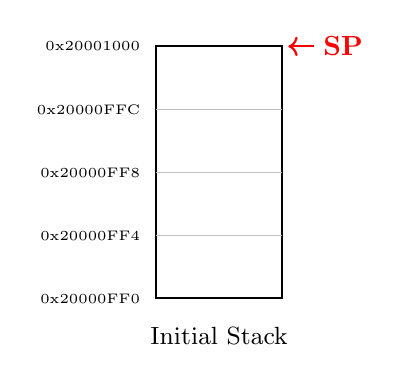
\begin{tikzpicture}[scale=0.8]
        % Stack frame
        \draw[thick] (0,0) rectangle (2,4);
        
        % Grid lines for 4 cells
        \foreach \y in {1,2,3} {
            \draw[thin, gray!50] (0,\y) -- (2,\y);
        }
        
        % Memory addresses (descending)
        \node[anchor=east] at (-0.1,4) {\tiny 0x20001000};
        \node[anchor=east] at (-0.1,3) {\tiny 0x20000FFC};
        \node[anchor=east] at (-0.1,2) {\tiny 0x20000FF8};
        \node[anchor=east] at (-0.1,1) {\tiny 0x20000FF4};
        \node[anchor=east] at (-0.1,0) {\tiny 0x20000FF0};
        
        % Stack pointer arrow
        \draw[->, thick, red] (2.5,4) -- (2.1,4);
        \node[right, red] at (2.5,4) {\textbf{SP}};
        
        % Title
        \node[below] at (1,-0.3) {\small Initial Stack};
    \end{tikzpicture}
    \caption{Initial empty stack}
    \label{fig:stack-initial}
\end{subfigure}
\hfill
\begin{subfigure}[t]{0.3\textwidth}
    \centering
    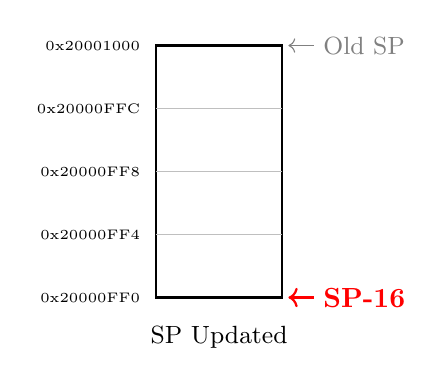
\begin{tikzpicture}[scale=0.8]
        % Stack frame
        \draw[thick] (0,0) rectangle (2,4);
        
        % Grid lines for 4 cells
        \foreach \y in {1,2,3} {
            \draw[thin, gray!50] (0,\y) -- (2,\y);
        }
        
        % Memory addresses (descending)
        \node[anchor=east] at (-0.1,4) {\tiny 0x20001000};
        \node[anchor=east] at (-0.1,3) {\tiny 0x20000FFC};
        \node[anchor=east] at (-0.1,2) {\tiny 0x20000FF8};
        \node[anchor=east] at (-0.1,1) {\tiny 0x20000FF4};
        \node[anchor=east] at (-0.1,0) {\tiny 0x20000FF0};
        
        % Old SP position (grayed out)
        \draw[->, thin, gray] (2.5,4) -- (2.1,4);
        \node[right, gray] at (2.5,4) {\small Old SP};
        
        % New SP position after PUSH {R0, R2, R4, LR}
        \draw[->, thick, red] (2.5,0) -- (2.1,0);
        \node[right, red] at (2.5,0) {\textbf{SP-16}};
        
        
        
        % Title
        \node[below] at (1,-0.3) {\small SP Updated};
    \end{tikzpicture}
    \caption{Stack pointer decremented}
    \label{fig:stack-sp-update}
\end{subfigure}
\hfill
\begin{subfigure}[t]{0.3\textwidth}
    \centering
    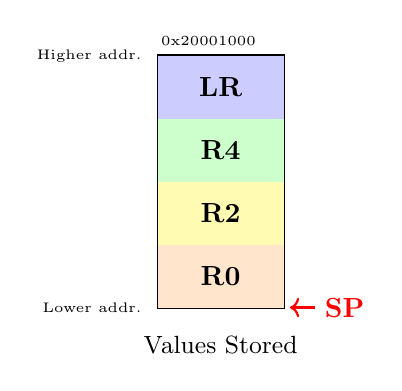
\begin{tikzpicture}[scale=0.8]
        % Stack frame
        \draw[thick] (0,0) rectangle (2,4);
        
        % Grid lines for 4 cells
        \foreach \y in {1,2,3} {
            \draw[thin, gray!50] (0,\y) -- (2,\y);
        }
        
        % Memory addresses (descending)
        \node[left, anchor=south west] at (-0.1,4) {\tiny 0x20001000};
        \node[left, anchor=south west] at (-0.1,3) {\tiny 0x20000FFC};
        \node[left, anchor=south west] at (-0.1,2) {\tiny 0x20000FF8};
        \node[left, anchor=south west] at (-0.1,1) {\tiny 0x20000FF4};
        \node[left, anchor=south west] at (-0.1,0) {\tiny 0x20000FF0};
        
        % Stored registers (in ascending order by number)
        \fill[blue!20] (0,3) rectangle (2,4);
        \node at (1,3.5) {\textbf{LR}};
        
        \fill[green!20] (0,2) rectangle (2,3);
        \node at (1,2.5) {\textbf{R4}};
        
        \fill[yellow!30] (0,1) rectangle (2,2);
        \node at (1,1.5) {\textbf{R2}};
        
        \fill[orange!20] (0,0) rectangle (2,1);
        \node at (1,0.5) {\textbf{R0}};
        
        % Stack pointer pointing to last used location
        \draw[->, thick, red] (2.5,0) -- (2.1,0);
        \node[right, red] at (2.5,0) {\textbf{SP}};
        
        % Annotations
        \node[left] at (-0.1,4) {\tiny Higher addr.};
        \node[left] at (-0.1,0) {\tiny Lower addr.};
        
        % Title
        \node[below] at (1,-0.3) {\small Values Stored};
    \end{tikzpicture}
    \caption{Registers stored in order}
    \label{fig:stack-values}
\end{subfigure}
\caption{Stack operation sequence for \texttt{PUSH \{R4, R0, R2, LR\}}}
\label{fig:stack-push-sequence}
\end{figure}

\noindent\textbf{Explanation:}
Figure~\ref{fig:stack-push-sequence}\textbf{(a)} shows the empty stack with \texttt{SP} at the top (highest address).
When \texttt{PUSH} executes, the processor \textbf{decrements \texttt{SP} by 16 bytes} to reserve space for four registers (Figure~\ref{fig:stack-push-sequence}\textbf{(b)}).
Finally, in Figure~\ref{fig:stack-push-sequence}\textbf{(c)}, values are stored according to the rule: the lowest-numbered register (R0) at the lowest address, then R2 and R4, and the highest-numbered (LR) at the highest address.
Because the stack grows downward, \texttt{SP} points to the last written word after the operation.

\bigskip
\paragraph{POP}

The \texttt{POP} instruction restores one or more registers from the stack.
Conceptually, the processor reads each value from the addresses currently covered by \texttt{SP} and then releases that stack space.
\textbf{Rule:} \texttt{POP} loads registers from the stack such that the \textbf{lowest-numbered register} is restored from the \textbf{lowest memory address}, and the \textbf{highest-numbered register} from the \textbf{highest memory address}.
After all specified registers are restored, \texttt{SP} has increased by 4 bytes per register.

\medskip
\noindent
\textbf{Example:}
\begin{lstlisting}
    POP {R6-R8}
\end{lstlisting}

This restores R6, then R7, then R8 from successively higher addresses; the stack pointer increases by 12 bytes overall.
If \texttt{PC} is included in the list, the loaded value becomes the new program counter, returning from the current procedure.

\begin{figure}[H]
\centering

\begin{subfigure}[t]{0.3\textwidth}
    \centering
    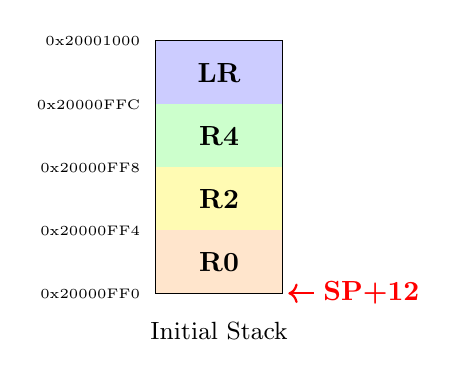
\begin{tikzpicture}[scale=0.8]
        % Stack frame
        \draw[thick] (0,0) rectangle (2,4);
        
        % Grid lines for 4 cells
        \foreach \y in {1,2,3} {
            \draw[thin, gray!50] (0,\y) -- (2,\y);
        }
        

        
        % Stored registers (in ascending order by number)
        \fill[blue!20] (0,3) rectangle (2,4);
        \node at (1,3.5) {\textbf{LR}};
        
        \fill[green!20] (0,2) rectangle (2,3);
        \node at (1,2.5) {\textbf{R4}};
        
        \fill[yellow!30] (0,1) rectangle (2,2);
        \node at (1,1.5) {\textbf{R2}};
        
        \fill[orange!20] (0,0) rectangle (2,1);
        \node at (1,0.5) {\textbf{R0}};
        
        % Stack pointer pointing to last used location
        \draw[->, thick, red] (2.5,0) -- (2.1,0);
        \node[right, red] at (2.5,0) {\textbf{SP+12}};
        
        % Annotations
        % Memory addresses (descending)
        \node[anchor=east] at (-0.1,4) {\tiny 0x20001000};
        \node[anchor=east] at (-0.1,3) {\tiny 0x20000FFC};
        \node[anchor=east] at (-0.1,2) {\tiny 0x20000FF8};
        \node[anchor=east] at (-0.1,1) {\tiny 0x20000FF4};
        \node[anchor=east] at (-0.1,0) {\tiny 0x20000FF0};
        
        % Title
        \node[below] at (1,-0.3) {\small Initial Stack};
    \end{tikzpicture}
    \caption{Initial stack after Figure \ref{fig:stack-push-sequence}}
\end{subfigure}
\hfill
\begin{subfigure}[t]{0.3\textwidth}
    \centering
    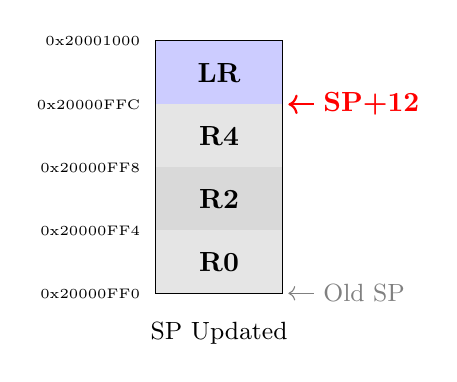
\begin{tikzpicture}[scale=0.8]
        % Stack frame
        \draw[thick] (0,0) rectangle (2,4);
        
        % Grid lines for 4 cells
        \foreach \y in {1,2,3} {
            \draw[thin, gray!50] (0,\y) -- (2,\y);
        }
        

        
        % Stored registers (in ascending order by number)
        \fill[blue!20] (0,3) rectangle (2,4);
        \node at (1,3.5) {\textbf{LR}};
        
        \fill[gray!20] (0,2) rectangle (2,3);
        \node at (1,2.5) {\textbf{R4}};
        
        \fill[gray!30] (0,1) rectangle (2,2);
        \node at (1,1.5) {\textbf{R2}};
        
        \fill[gray!20] (0,0) rectangle (2,1);
        \node at (1,0.5) {\textbf{R0}};
        
        % Stack pointer pointing to last used location
        \draw[->, thin, gray] (2.5,0) -- (2.1,0);
        \node[right, gray] at (2.5,0) {\small{Old SP}}; 

        \draw[->, thick, red] (2.5,3) -- (2.1,3);
        \node[right, red] at (2.5,3) {\textbf{SP+12}};
        
        % Annotations
        % Memory addresses (descending)
        \node[anchor=east] at (-0.1,4) {\tiny 0x20001000};
        \node[anchor=east] at (-0.1,3) {\tiny 0x20000FFC};
        \node[anchor=east] at (-0.1,2) {\tiny 0x20000FF8};
        \node[anchor=east] at (-0.1,1) {\tiny 0x20000FF4};
        \node[anchor=east] at (-0.1,0) {\tiny 0x20000FF0};
        
        % Title
        \node[below] at (1,-0.3) {\small SP Updated};
    \end{tikzpicture}
    \caption{Stack pointer incremented}
\end{subfigure}
\hfill
\begin{subfigure}[t]{0.3\textwidth}
    \centering
    \centering
    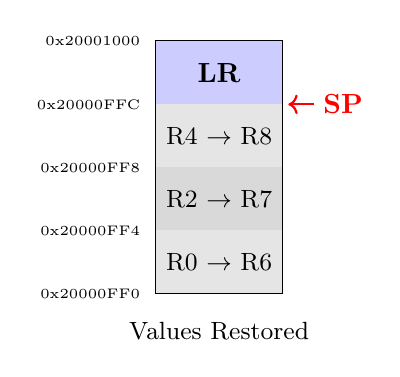
\begin{tikzpicture}[scale=0.8]
        % Stack frame
        \draw[thick] (0,0) rectangle (2,4);
        
        % Grid lines for 4 cells
        \foreach \y in {1,2,3} {
            \draw[thin, gray!50] (0,\y) -- (2,\y);
        }
        

        
        % Stored registers (in ascending order by number)
        \fill[blue!20] (0,3) rectangle (2,4);
        \node at (1,3.5) {\textbf{LR}};
        
        \fill[gray!20] (0,2) rectangle (2,3);
        \node at (1,2.5) {\small{R4 $\rightarrow$ R8}};
        
        \fill[gray!30] (0,1) rectangle (2,2);
        \node at (1,1.5) {\small{R2 $\rightarrow$ R7}};

        \fill[gray!20] (0,0) rectangle (2,1);
        \node at (1,0.5) {\small{R0 $\rightarrow$ R6}};
        
        % Stack pointer pointing to last used location
        \draw[->, thick, red] (2.5,3) -- (2.1,3);
        \node[right, red] at (2.5,3) {\textbf{SP}};
        
        % Annotations
        % Memory addresses (descending)
        \node[anchor=east] at (-0.1,4) {\tiny 0x20001000};
        \node[anchor=east] at (-0.1,3) {\tiny 0x20000FFC};
        \node[anchor=east] at (-0.1,2) {\tiny 0x20000FF8};
        \node[anchor=east] at (-0.1,1) {\tiny 0x20000FF4};
        \node[anchor=east] at (-0.1,0) {\tiny 0x20000FF0};
        
        % Title
        \node[below] at (1,-0.3) {\small Values Restored};
    \end{tikzpicture}
    \caption{Registers restored in order}
    \label{fig:stack-sp-update}
\end{subfigure}

\caption{Stack operation sequence for \texttt{POP \{R6-R8\}}}
\label{fig:stack-pop-sequence}
\end{figure}
\noindent\textbf{Explanation:}
In Figure~\ref{fig:stack-pop-sequence}\textbf{(a)}, the stack contains values saved earlier.
Executing \texttt{POP \{R6-R8\}} \textbf{reclaims 12 bytes of stack space} (three registers) by moving \texttt{SP} upward in memory (Figure~\ref{fig:stack-pop-sequence}\textbf{(b)}).
Then, as shown in Figure~\ref{fig:stack-pop-sequence}\textbf{(c)}, registers are restored following the rule: the lowest-numbered register (R6) comes from the lowest address, followed by R7 and R8 from higher addresses.
After the last load, \texttt{SP} points to the top of the reclaimed block, completing the reversal of the earlier push.



\newpage
\section{Procedure}

\subsection{Examples}

\subsubsection{Example 1: Array Example — Find Maximum Element}
This example demonstrates how to find the maximum element in an array using a standard for loop structure.
\lstinputlisting[caption={Find maximum element in an array}]{snippets/assembly/exp3/example1.asm}
\paragraph{Check:} Verify that the maximum element is correctly identified and stored in \texttt{MAXRES}.
\newpage

\subsubsection{Example 2: String Example — Count Uppercase Letters}
This example demonstrates how to process a null-terminated string and count the number of uppercase letters (A-Z) using a while-loop structure.
\lstinputlisting[caption={Count uppercase letters in a string}]{snippets/assembly/exp3/example2.asm}
\paragraph{Check:} Verify that the program correctly counts the uppercase letters and stores the result in \texttt{UPPERCOUNT}.

\newpage
\subsubsection{Example 3: Stack Example — Nested Uppercase Counter}
This example demonstrates a nested call: \texttt{CountUpperNested(ptr)} scans a null-terminated string and calls \texttt{IsUpper(ch)} for each character. It shows saving/restoring \texttt{LR} and using a callee-saved register (\texttt{R4}) for the running count.
\lstinputlisting[caption={Nested procedure call to count uppercase letters}]{snippets/assembly/exp3/example3.asm}
\paragraph{Check:} Verify that \texttt{UPPERCOUNT} contains \texttt{5} for the test string.

\newpage
\subsection{Tasks}

\subsubsection{Task 1: Count Vowels in a String}
Implement procedures to process strings with the following requirements:
\begin{itemize}[nosep]
    \item Create a procedure \texttt{CountVowels} that takes a string pointer in R0 and returns the number of vowels (a, e, i, o, u) in R0.
    \item Use nested procedure calls where \texttt{CountVowels} calls a helper procedure \texttt{IsVowel}.
    \item Follow AAPCS conventions for parameter passing and register usage.
\end{itemize}

\subsubsection{Task 2: Factorial Calculation (Iterative)}
Implement a procedure to calculate the factorial of a non-negative integer:
\begin{itemize}[nosep]
    \item Create a procedure \texttt{Factorial} that takes a non-negative integer in R0 and returns its factorial in R0.
    \item Use an iterative approach with a loop to compute the factorial.
    \item Ensure proper handling of edge cases, such as 0! = 1.
    \item Follow AAPCS conventions for parameter passing and register usage.
\end{itemize}
\subsubsection{Task 3: Factorial Calculation (Recursive)}
Implement a recursive version of the factorial calculation:
\begin{itemize}[nosep]
    \item Create a procedure \texttt{FactorialRec} that takes a non-negative integer in R0 and returns its factorial in R0.
    \item Use recursion to compute the factorial, ensuring proper base case handling.
    \item Manage the stack appropriately to save and restore registers as needed.
    \item Follow AAPCS conventions for parameter passing and register usage.
    \item Test the procedure with various inputs to verify correctness.
\end{itemize}
\toconlypart{EK-TM4C123GXL Board and Peripherals}
\chapter{TM4C123 Microcontroller: Architecture and Digital Outputs}

\section*{Learning Objectives}
After completing this experiment, you will be able to:
\begin{itemize}[nosep]
  \item Identify the main components and subsystems of the TM4C123 microcontroller and understand their roles within an embedded system.
  \item Recognize the organization of the ARM Cortex-M4 core, memory map, and peripheral buses.
  \item Understand the role of core peripherals including NVIC, SysTick, and System Control Block (SCB).
  \item Configure and control digital output pins using the General-Purpose Input/Output (GPIO) module.
  \item Write Assembly programs to drive on-board LEDs through direct register access.
  \item Relate register operations to physical hardware behavior and verify functionality through observation on the LaunchPad board.
\end{itemize}

\section*{Experiment Overview}
This experiment introduces the architecture of the TM4C123 microcontroller and its most fundamental feature — the ability to interface with the outside world through digital I/O pins.

\noindent You will first explore the internal structure of the device, including the ARM Cortex-M4 core, core peripherals (NVIC, SysTick, SCB), buses, memory regions, and peripheral interconnect. Then, you will apply this understanding by writing Assembly programs that toggle the on-board LEDs connected to \texttt{PORTF}.

\noindent In this experiment, you will:
\begin{itemize}[nosep]
  \item Understand how peripheral registers are mapped into memory and accessed by the CPU.
  \item Learn about Cortex-M4 core peripherals and their functions.
  \item Learn the initialization sequence required to enable and configure GPIO ports.
  \item Develop Assembly programs that control LEDs using software delays.
  \item Form the foundation for subsequent experiments involving interrupts, timers, and analog peripherals.
\end{itemize}

By the end of this lab, you will understand the TM4C123 architecture, Cortex-M4 core peripherals, be able to configure GPIO ports for digital output, and control external hardware through register manipulation in Assembly.

\newpage
\etocsetnexttocdepth{subsubsection}
\localtableofcontents
\bigskip
\newpage

\section{Theoretical Background}

\subsection{TM4C123 Microcontroller Architecture}

The TM4C123GH6PM microcontroller is built around the ARM Cortex-M4F processor core, implementing the ARMv7-M architecture. It integrates the CPU core, memory, peripherals, and I/O interfaces on a single chip — a complete system-on-chip (SoC) solution for embedded applications.

\subsubsection{Core Components}

The TM4C123 contains the following major components:
\begin{itemize}[nosep]
  \item \textbf{ARM Cortex-M4F Processor Core}: 32-bit RISC processor with hardware Floating-Point Unit (FPU)
  \item \textbf{Memory}: 256 KB Flash, 32 KB SRAM, 2 KB EEPROM
  \item \textbf{System Buses}: Advanced High-Performance Bus (AHB) and Advanced Peripheral Bus (APB)
  \item \textbf{Core Peripherals}: NVIC, SysTick Timer, Memory Protection Unit (MPU), System Control Block (SCB)
  \item \textbf{General-Purpose Timers}: Six 16/32-bit and six 32/64-bit timers
  \item \textbf{Communication Interfaces}: UART, I\textsuperscript{2}C, SSI (SPI), CAN
  \item \textbf{Analog Peripherals}: 12-bit ADC with 12 channels, analog comparators
  \item \textbf{GPIO Ports}: Six ports (A-F) with up to 43 programmable pins
\end{itemize}

\subsection{ARM Cortex-M4 Core Peripherals}

The ARM Cortex-M4 processor includes several \textbf{core peripherals} that are common across all Cortex-M4-based microcontrollers.  
They are tightly integrated with the CPU and provide essential system functions such as interrupt handling and timing.

\subsubsection{Nested Vectored Interrupt Controller (NVIC)}

The NVIC manages all interrupt and exception handling.  
It supports up to 240 interrupt sources (138 on the TM4C123), hardware priority levels, and automatic context saving for efficient servicing.  
Key features include nesting, tail-chaining, and late-arrival handling for minimal interrupt latency.

\noindent Important NVIC registers (base address \texttt{0xE000E100}):
\begin{itemize}[nosep]
  \item \texttt{NVIC\_ENx} — Set-Enable  
  \item \texttt{NVIC\_DISx} — Clear-Enable  
  \item \texttt{NVIC\_PRIx} — Priority Configuration  
  \item \texttt{NVIC\_ACTIVEx} — Active Status
\end{itemize}

\subsubsection{SysTick Timer}

The SysTick timer is a simple 24-bit down-counter integrated in the core.  
It provides a consistent time base for system delays or periodic tasks.  
Many operating systems use it for time-keeping or scheduling.

\noindent SysTick registers (base address \texttt{0xE000E010}):
\begin{itemize}[nosep]
  \item \texttt{STCTRL} — Control and Status  
  \item \texttt{STRELOAD} — Reload Value  
  \item \texttt{STCURRENT} — Current Counter Value
\end{itemize}

\noindent Other core peripherals such as the System Control Block (SCB) are present but not covered in this course.
\bigskip

\subsection{Memory Map}

The Cortex-M4 processor uses a unified 4 GB address space for all code, data, and peripherals.  
Every peripheral and memory region occupies a unique address range, allowing direct access through normal load and store instructions.

\begin{table}[H]
\centering
\small
\begin{tabular}{lll}
\toprule
\textbf{Region} & \textbf{Address Range} & \textbf{Description} \\
\midrule
Flash Memory & 0x00000000 - 0x0003FFFF & Program storage (256 KB) \\
SRAM & 0x20000000 - 0x20007FFF & On-chip data memory (32 KB) \\
Peripherals & 0x40000000 - 0x400FFFFF & Peripheral registers \\
GPIO Ports & 0x40004000 - 0x40025FFF & GPIO A-F registers \\
Core Peripherals & 0xE0000000 - 0xE00FFFFF & NVIC, SysTick, SCB, etc. \\
\bottomrule
\end{tabular}
\caption{Simplified TM4C123 Memory Map}
\end{table}

\noindent
Each peripheral's registers are \textbf{memory-mapped}, meaning they are accessed just like variables in memory.  
For example, writing to address \texttt{0x400253FC} directly updates the GPIO Port F data register.


\subsection{General-Purpose Input/Output (GPIO)}

GPIO (General-Purpose Input/Output) ports form the primary interface between the microcontroller and external devices such as LEDs, switches, and sensors. Each pin can be configured as either an input or an output.

When a pin is an \textbf{output}, software drives it high or low to control external hardware (e.g., turn an LED on/off).  
When a pin is an \textbf{input}, software reads its logic level (e.g., a button press).

\subsubsection{GPIO Ports Overview}

The TM4C123GH6PM provides six GPIO ports (A-F), each with up to eight programmable pins. Not all pins are available on the LaunchPad, and some are reserved for debugging or special functions.

\begin{table}[H]
\centering
\small
\renewcommand{\arraystretch}{1.2}
\begin{tabular}{cll}
\toprule
\textbf{Port} & \textbf{Pins Available} & \textbf{Notes} \\
\midrule
Port A & PA0-PA7 & UART0 (PA0, PA1) shared with USB debug interface \\
Port B & PB0-PB7 & I\textsuperscript{2}C0, SSI2, ADC channels \\
Port C & PC0-PC7 & PC0-PC3 used for JTAG (avoid modification) \\
Port D & PD0-PD7 & PD7 requires unlock for GPIO use \\
Port E & PE0-PE5 & ADC and UART5 functionality available \\
Port F & PF0-PF4 & On-board LEDs (PF1-PF3) and switches (PF0, PF4) \\
\bottomrule
\end{tabular}
\caption{GPIO Port Summary — TM4C123GH6PM}
\end{table}

\noindent
Each port exposes its own control and data registers, allowing independent configuration and operation.
\bigskip

\subsubsection{Memory-Mapped GPIO Registers}

GPIO modules are accessed via \textbf{memory-mapped registers}: fixed addresses that the CPU reads/writes with standard \texttt{LDR}/\texttt{STR} instructions.

\noindent
Every port has a \textbf{base address}; key registers sit at fixed offsets from that base.

\begin{table}[H]
\centering
\small
\begin{tabular}{cl}
\toprule
\textbf{Port} & \textbf{Base Address} \\
\midrule
Port A & 0x40004000 \\
Port B & 0x40005000 \\
Port C & 0x40006000 \\
Port D & 0x40007000 \\
Port E & 0x40024000 \\
Port F & 0x40025000 \\
\bottomrule
\end{tabular}
\caption{GPIO Port Base Addresses (TM4C123GH6PM)}
\end{table}

\noindent
In this experiment we use Port~F, so:
\[
\texttt{GPIODIR} = \texttt{0x40025400},\quad
\texttt{GPIODEN} = \texttt{0x4002551C},\quad
\texttt{GPIODATA} = \texttt{0x400253FC}.
\]
\bigskip

\subsubsection{Address Masking in \texttt{GPIODATA}}

The \texttt{GPIODATA} register supports \textbf{address masking}: address bits [9:2] form a bit mask that selects which pins are affected.

\begin{itemize}[nosep]
  \item \textbf{Full access:} Base + \texttt{0x3FC} — all 8 pins.
  \item \textbf{Masked access:} Base + (\texttt{mask} $\ll$ 2) — only the pins in \texttt{mask}.
\end{itemize}

\noindent
Example (PF1 only):
\[
\texttt{0x40025000 + (0x02 << 2) = 0x40025008}.
\]
This is \textbf{address masking} (often confused with “bit-banding”); it enables fast, selective reads/writes to individual pins.
\bigskip

\subsubsection{Protected and Special-Function Pins}

Some pins are locked or reserved at reset due to critical roles:

\begin{itemize}[nosep]
  \item \textbf{PF0} doubles as the Non-Maskable Interrupt (NMI) input and is locked. To use it as GPIO, write \texttt{0x4C4F434B} to \texttt{GPIO\_LOCK} and set the desired bits in \texttt{GPIO\_CR}.
  \item \textbf{PC0-PC3} carry the JTAG debug interface and should not be reassigned in normal operation.
\end{itemize}

\noindent
Always confirm pin availability in the datasheet before repurposing special-function pins.
\bigskip

\subsubsection{Port F on the LaunchPad}

Port~F connects to the on-board RGB LEDs and user push buttons:

\begin{table}[H]
\centering
\small
\renewcommand{\arraystretch}{1.2}
\begin{tabular}{clll}
\toprule
\textbf{Pin} & \textbf{Function} & \textbf{Connected Component} & \textbf{Active Level} \\
\midrule
PF1 & Output & Red LED & Active High \\
PF2 & Output & Blue LED & Active High \\
PF3 & Output & Green LED & Active High \\
PF0 & Input (locked) & SW2 (Push Button) & Active Low (enable pull-up) \\
PF4 & Input & SW1 (Push Button) & Active Low (enable pull-up) \\
\bottomrule
\end{tabular}
\caption{GPIO Port F Pin Assignments — TM4C123 LaunchPad}
\end{table}

\noindent
LEDs are \textbf{active-high} (write 1 to turn on). Push buttons pull to ground when pressed, so inputs read \textbf{0 when pressed} and require internal pull-ups.
\bigskip

\subsubsection{GPIO Configuration Workflow}

In practice, GPIO usage has two phases:

\begin{itemize}[nosep]
  \item \textbf{Initialization (setup, runs once):} enable the port clock, unlock protected pins (if needed), set direction, and enable digital function.
  \item \textbf{Runtime (operation, repeats):} read inputs or write outputs by accessing \texttt{GPIODATA} in the main loop or in interrupt service routines (ISRs).
\end{itemize}

\noindent
A typical structure is:

\begin{lstlisting}[language=C,caption={Typical GPIO program structure (setup vs. runtime)}]
InitGPIO();                // RCGCGPIO, optional LOCK/CR, DIR, DEN
while (1) {                // Runtime phase
    // Read buttons (inputs) and/or drive LEDs (outputs)
    // Optionally, some I/O is handled inside ISRs
}
\end{lstlisting}

\medskip
\noindent
The detailed register-level steps (clock enable, unlock, direction, digital enable, and data access) are demonstrated in the following subsections.

\newpage
\subsubsection*{Step 1 — Enable the GPIO Port Clock}

\noindent\textbf{Register:} \texttt{RCGCGPIO} — Run Mode Clock Gating Control for GPIO (\texttt{0x400FE608})

\noindent
Before accessing any GPIO port, its clock must be enabled.  
The \texttt{RCGCGPIO} register controls the clock to all GPIO modules.  
Each bit corresponds to a single port (A-F). Writing a '1' to a bit enables the clock to that port, while '0' disables it.

\begin{figure}[H]
\centering
\begin{bytefield}[bitwidth=1.1em,bitheight=2.7ex,
                  boxformatting={\centering\small},
                  endianness=big, bitwidth=\widthof{\tiny~PF~}]{32}
\bitheader{31,5,4,3,2,1,0}\\
\bitbox{26}[bgcolor=gray!10]{\textit{Reserved}} &
\bitbox{1}{\tiny{PF}} &
\bitbox{1}{\tiny{PE}} &
\bitbox{1}{\tiny{PD}} &
\bitbox{1}{\tiny{PC}} &
\bitbox{1}{\tiny{PB}} &
\bitbox{1}{\tiny{PA}}
\end{bytefield}
\caption{RCGCGPIO Register (\texttt{0x400FE608}) — GPIO Clock Control}
\end{figure}

\noindent
To activate Port~F, bit~5 must be set to~1 as shown below.

\begin{lstlisting}[caption={Enable clock for Port F}]
        LDR     R1, =0x400FE608     ; RCGCGPIO register
        LDR     R0, [R1]
        ORR     R0, R0, #0x20       ; Set bit 5 (Port F)
        STR     R0, [R1]
\end{lstlisting}
\noindent
Once the clock is enabled, a short delay or status polling ensures the peripheral is ready before further configuration.
\bigskip


\subsubsection*{Step 2 — Unlock Protected Pins}
\noindent\textbf{Registers:} \texttt{GPIO\_LOCK} (\texttt{0x40025520}), \texttt{GPIO\_CR} (\texttt{0x40025524})

\noindent
Certain pins such as PF0 are protected because they share critical alternate functions (e.g., the NMI input).  
To modify these pins, the port must be unlocked by writing the key value \texttt{0x4C4F434B} (“LOCK”) into the \texttt{GPIO\_LOCK} register.  
The \texttt{GPIO\_CR} register (Commit Register) then determines which pins can be altered.

\begin{figure}[H]
\centering
\begin{bytefield}[bitheight=2.7ex,
  boxformatting={\centering\small},endianness=big, bitwidth=\widthof{\tiny~PF~}]{32}
\bitheader{31,8,7,0}\\
\bitbox{24}[bgcolor=gray!10]{\textit{Reserved}} &
\bitbox{8}{\tiny Commit Mask}
\end{bytefield}
\caption{GPIO\_CR Register — Commit Control}
\end{figure}

\noindent
The following code unlocks Port~F and enables modification of all pins.

\begin{lstlisting}[caption={Unlock Port F}]
        LDR     R1, =0x40025520     ; GPIO_LOCK
        LDR     R0, =0x4C4F434B     ; Unlock key
        STR     R0, [R1]            
        LDR     R1, =0x40025524     ; GPIO_CR
        MOV     R0, #0xFF           ; Allow changes to all pins
        STR     R0, [R1]
\end{lstlisting}
\noindent
In this experiment, PF0 is not used, so unlocking is optional. After unlocking, configuration registers such as direction and digital enable can be safely modified.
\bigskip


\subsubsection*{Step 3 — Configure Pin Direction}
\noindent\textbf{Register:} \texttt{GPIODIR} (\texttt{0x40025400}) — GPIO Direction Control (Port~F)

\noindent
The \texttt{GPIODIR} register determines whether each GPIO pin functions as an input or an output.  
Writing '0' configures the pin as an input, while '1' configures it as an output.

\begin{figure}[H]
\centering
\begin{bytefield}[bitwidth=\widthof{\tiny~PF~},bitheight=2.7ex,
  boxformatting={\centering\small},endianness=big]{32}
\bitheader{31,8,7,6,5,4,3,2,1,0}\\
\bitbox{24}[bgcolor=gray!10]{\textit{Reserved}} &
\bitbox{1}{\tiny F7} &
\bitbox{1}{\tiny F6} &
\bitbox{1}{\tiny F5} &
\bitbox{1}{\tiny F4} &
\bitbox{1}{\tiny F3} &
\bitbox{1}{\tiny F2} &
\bitbox{1}{\tiny F1} &
\bitbox{1}{\tiny F0}
\end{bytefield}
\caption{GPIODIR Register (Port F) — Direction Control}
\end{figure}

\noindent
For the on-board RGB LED, PF1-PF3 must be configured as outputs.  
Bits 1-3 are therefore set to '1'.

\begin{lstlisting}[caption={Set PF1, PF2, PF3 as outputs}]
        LDR     R1, =0x40025400     ; GPIODIR register (Port F)
        LDR     R0, [R1]
        ORR     R0, R0, #0x0E       ; Set PF1, PF2, PF3 as outputs
        STR     R0, [R1]
\end{lstlisting}
\noindent
Unmodified bits remain unchanged, allowing input pins (such as PF0 or PF4) to retain their default configuration.
\bigskip


\subsubsection*{Step 4 — Enable Digital Functionality}
\noindent\textbf{Register:} \texttt{GPIODEN} (\texttt{0x4002551C}) — Digital Enable Register (Port~F)

\noindent
Each GPIO pin can serve analog or digital functions.  
The \texttt{GPIODEN} register enables the digital circuitry for selected pins.  
Pins configured as digital inputs or outputs must have their corresponding bits set to '1'.

\begin{figure}[H]
\centering
\begin{bytefield}[bitwidth=\widthof{\tiny~PF~},bitheight=2.7ex,
  boxformatting={\centering\small},endianness=big]{32}
\bitheader{31,8,7,6,5,4,3,2,1,0}\\
\bitbox{24}[bgcolor=gray!10]{\textit{Reserved}} &
\bitbox{1}{\tiny F7} &
\bitbox{1}{\tiny F6} &
\bitbox{1}{\tiny F5} &
\bitbox{1}{\tiny F4} &
\bitbox{1}{\tiny F3} &
\bitbox{1}{\tiny F2} &
\bitbox{1}{\tiny F1} &
\bitbox{1}{\tiny F0}
\end{bytefield}
\caption{GPIODEN Register (Port F) — Digital Enable}
\end{figure}

\noindent
Bits~1-3 are set to enable PF1-PF3 as digital outputs for the LED.

\begin{lstlisting}[caption={Enable digital function for PF1-PF3}]
        LDR     R1, =0x4002551C     ; GPIODEN register (Port F)
        LDR     R0, [R1]
        ORR     R0, R0, #0x0E       ; Enable PF1-PF3 as digital pins
        STR     R0, [R1]
\end{lstlisting}
\noindent
Failing to enable \texttt{GPIODEN} leaves the pins electrically inactive even if their direction is set.
\bigskip


\subsubsection*{Step 5 — Write to the Data Register}
\noindent\textbf{Register:} \texttt{GPIODATA} (\texttt{0x400253FC}) — Data Input/Output Register (Port~F)

\noindent
The \texttt{GPIODATA} register reflects the current logic levels on all GPIO pins.  
Writing to a bit drives the corresponding output high ('1') or low ('0').  
Bits 1-3 correspond to the RGB LED pins on the LaunchPad:  
PF1 = Red, PF2 = Blue, PF3 = Green.

\begin{figure}[H]
\centering
\begin{bytefield}[bitwidth=\widthof{\tiny ~PF~},bitheight=2.7ex,
  boxformatting={\centering\small},endianness=big]{32}
\bitheader{31,8,7,6,5,4,3,2,1,0}\\
\bitbox{24}[bgcolor=gray!10]{\textit{Reserved}} &
\bitbox{1}{\tiny F7} &
\bitbox{1}{\tiny F6} &
\bitbox{1}{\tiny F5} &
\bitbox{1}{\tiny F4} &
\bitbox{1}{\tiny F3} &
\bitbox{1}{\tiny F2} &
\bitbox{1}{\tiny F1} &
\bitbox{1}{\tiny F0}
\end{bytefield}
\caption{GPIODATA Register (Port F) — Data Output/Input}
\end{figure}

\noindent
The example below drives PF1 (Red) and PF3 (Green) simultaneously to produce a yellow color.

\begin{lstlisting}[caption={Turn on Yellow LED (Red + Green = PF1 + PF3)}]
    LDR     R1, =0x400253FC     ; GPIODATA register (Port F)
    MOV     R0, #0x0A           ; Set PF1 (Red) and PF3 (Green) = Yellow
    STR     R0, [R1]
\end{lstlisting}
\noindent
By writing different bit combinations, various LED colors can be generated:
\newcommand{\ledon}[1]{\tikz\fill[#1,draw=black] (0,0) circle (0.6ex);}
\newcommand{\ledoff}{\tikz\draw[gray!70] (0,0) circle (0.6ex);}

\begin{table}[H]
\centering
\small

\renewcommand{\arraystretch}{1.2}
\begin{tabular}{lccccl}
\toprule
\textbf{Color} & \textbf{Red (PF1)} & \textbf{Blue (PF2)} & \textbf{Green (PF3)} & \textbf{Hex} & \textbf{Combination} \\
\midrule
Red      & \ledon{red}    & \ledoff & \ledoff & 0x02 & Red only \\
Blue     & \ledoff        & \ledon{blue} & \ledoff & 0x04 & Blue only \\
Green    & \ledoff        & \ledoff & \ledon{green!70!black} & 0x08 & Green only \\
Yellow   & \ledon{red}    & \ledoff & \ledon{green!70!black} & 0x0A & Red + Green \\
Cyan     & \ledoff        & \ledon{blue} & \ledon{green!70!black} & 0x0C & Blue + Green \\
Magenta  & \ledon{red}    & \ledon{blue} & \ledoff & 0x06 & Red + Blue \\
White    & \ledon{red}    & \ledon{blue} & \ledon{green!70!black} & 0x0E & All on \\
\bottomrule
\end{tabular}
\caption{LED Color Combinations on TM4C123 LaunchPad (PF1-PF3)}
\label{tab:led-colors}
\end{table}
\newpage
\section{Procedure}
\subsection{Examples}
The following examples illustrate the complete process of initializing Port~F and controlling the on-board LEDs using Assembly language.
\subsubsection{Example 1 — Simple LED Blink}
This example initializes Port~F and toggles the Red LED (PF1) on and off using address masking with a software delay.
Address Masking for PF1:
\[
\texttt{0x40025000 + (0x02 << 2) = 0x40025008}
\]
\Needspace{37\baselineskip} % reserve space for the block; else start a new page
\lstinputlisting[caption={Assembly code to blink the Red LED (PF1) on the TM4C123 LaunchPad}]{snippets/gpio/example1.asm}

\subsubsection{Example 2 — Cycle Through RGB Colors}
This example extends the previous one by cycling through RGB LED colors (Red, Green, Blue) using a software delay.
Address Masking for PF1, PF2, PF3:
\[
\texttt{0x40025000 + ((0x02 | 0x04 | 0x08) << 2) = 0x40025038}
\]
\Needspace{55\baselineskip} % reserve space for the block; else start a new page
\lstinputlisting[caption={Assembly code to cycle through RGB colors on the TM4C123 LaunchPad}]{snippets/gpio/example2.asm}
\subsection{Tasks}

\subsubsection{Task 1 — Adjust the Blink Rate}
Modify the delay routine in \textbf{Example 1} to change the blinking speed of the Red LED.  
Experiment with different delay values until the LED blinks at approximately \textbf{1 Hz} (about one second ON and one second OFF).

\medskip

\subsubsection{Task 2 — Cycle Through Multiple Colors}
Expand \textbf{Example 2} to include additional colors by combining the Red, Green, and Blue LEDs.  
Create a program that automatically cycles through all color combinations listed in Table~\ref{tab:led-colors}. \\

\smallskip

\noindent\textit{Hint:} Use a loop to step through the color sequence repeatedly instead of writing separate code for each color.

\chapter{Interrupt Handling and the Nested Vectored Interrupt Controller}
\chapter{System Timers and General-Purpose Timer Modules}
\chapter{Liquid Crystal Display Interfacing and Control}
\chapter{Analog-to-Digital Conversion (ADC)}
\chapter{UART Serial Communication}

\clearpage
\ifodd\value{page}
  % already odd: do nothing
\else
  \thispagestyle{empty}\null\newpage
\fi
\end{document}

